% Paquets généraux
\documentclass[a4paper,12pt,titlepage,twoside]{article}
\usepackage[T1]{fontenc}
\usepackage[utf8]{inputenc}
\usepackage[french]{babel}
\usepackage{subcaption}
\addto\captionsfrench{%
  \renewcommand{\tablename}{Tableau}%
}
\usepackage[gen]{eurosym}
%\usepackage[dvips]{graphicx}
\usepackage{minted}
\usepackage{fancyhdr}
\usepackage{pdfpages} 
\usepackage{multido}
\usepackage{hyperref}
\usepackage{textcomp}
\usepackage{schemabloc}
%\usepackage[bitstream-charter]{mathdesign}
\usepackage{array}
\newcolumntype{P}[1]{>{\centering\arraybackslash}p{#1}}
\usepackage[shortlabels]{enumitem}
\usepackage[framemethod=TikZ]{mdframed}

\newcommand{\id}{71}
\newcommand{\nom}{Théorie des mécanismes}
\newcommand{\sequence}{04}
\newcommand{\nomsequence}{Liaisons entre les solides}
\newcommand{\num}{02}
\newcommand{\type}{KH}
\newcommand{\descrip}{Liaisons équivalentes, hyperstatisme, liaisons en série et en parallèle, théorie des graphes}
\newcommand{\competences}{B2-12: Proposer une modélisation des liaisons avec leurs caractéristiques géométriques. \\ &  B2-13: Proposer un modèle cinématique paramétré à partir d'un système réel, d'une maquette numérique ou d'u \\ &  B2-17: Simplifier un modèle de mécanisme. \\ &  B2-18: Modifier un modèle pour le rendre isostatique. \\ &  C1-04: Proposer une démarche permettant d'obtenir une loi entrée-sortie géométrique.  \\ &  C2-05: Caractériser le mouvement d'un repère par rapport à un autre repère. \\ &  C2-06: Déterminer les relations entre les grandeurs géométriques ou cinématiques. }
\newcommand{\nbcomp}{7}
\newcommand{\systemes}{}
\newcommand{\systemesnum}{}
\newcommand{\systemessansaccent}{}
\newcommand{\ilot}{2}
\newcommand{\ilotstr}{02}
\newcommand{\dossierilot}{\detokenize{Ilot_02 }}

%\usepackage{style}
\usepackage{bodegraph}
\usepackage{rpcinematik}
\usepackage[locale = FR]{siunitx}
\usepackage{caption}
\newcommand{\institute}{Lycée Dorian}

\usepackage{listings}
\usepackage{fancyvrb}
\usepackage{color}
\usepackage{xcolor}
\usepackage{colortbl}
\usepackage{helvet}
\usepackage[frenchmath]{newtxsf} % for sans serif symbols
\renewcommand{\familydefault}{\sfdefault}
%\usepackage{amsfonts}
%\usepackage{amsmath}
%\usepackage{lmodern}
\usepackage{mathastext}
%\usepackage{xspace}
\usepackage{varioref}
\usepackage{tabularx}
%\usepackage{floatflt}
\usepackage{graphics}
\usepackage{wrapfig}
\usepackage{textcomp}
\usepackage{tikz,tkz-tab}
\usepackage[european resistor, european voltage, european current]{circuitikz}
\usepackage{wrapfig}
\usepackage{gensymb}
\usepackage[percent]{overpic}
\usetikzlibrary{babel}
\usepackage{ifthen}
\usepackage{cancel}
\usepackage{etoolbox}
\usepackage{multirow}
%\usepackage{boxedminipage}
\definecolor{gris25}{gray}{0.75}
\definecolor{bleu}{RGB}{18,33,98}
\definecolor{bleuf}{RGB}{42,94,171}
\definecolor{bleuc}{RGB}{231,239,247}
\definecolor{bleum}{RGB}{160,195,226}
\definecolor{rougef}{RGB}{185,18,27}
\definecolor{rougec}{RGB}{255,188,204}%255,230,231
\definecolor{vertf}{RGB}{103,126,82}
\definecolor{vertc}{RGB}{220,255,191}
\definecolor{forestgreen}{rgb}{0.13,0.54,0.13}
\definecolor{blcr}{rgb}{0.59,0.69,0.84}
\definecolor{blfr}{rgb}{0.32,0.51,0.75}
\definecolor{orfr}{rgb}{0.90,0.42,0.15}
\definecolor{orcr}{rgb}{0.90,0.65,0.50}
\definecolor{orangef}{rgb}{0.659,0.269,0.072}
\definecolor{orange}{rgb}{0.58,0.35,0.063}
\definecolor{orangec}{rgb}{0.43,0.32,0.25}
\definecolor{rcorrect}{rgb}{0.6,0,0}
\definecolor{sequence}{rgb}{0.75,0.75,0.75}
\definecolor{competences}{rgb}{0.61,0.73,0.35}
\definecolor{rose}{HTML}{ff00ff}
\definecolor{grisf}{HTML}{222222}
\definecolor{grisc}{HTML}{636363}
\definecolor{normal}{HTML}{4087c4}
\definecolor{info}{HTML}{5bc0de}
\definecolor{success}{RGB}{92,184,92}
\definecolor{warning}{RGB}{240,173,78}
\definecolor{danger}{RGB}{217,83,79}
\hypersetup{                    % parametrage des hyperliens
    colorlinks=true,                % colorise les liens
    breaklinks=true,                % permet les retours à la ligne pour les liens trop longs
    urlcolor= blfr,                 % couleur des hyperliens
    linkcolor= orange,                % couleur des liens internes aux documents (index, figures, tableaux, equations,...)
    citecolor= forestgreen                % couleur des liens vers les references bibliographiques
    }

\newcolumntype{M}[1]{>{\centering\arraybackslash}m{#1}}
\definecolor{codegreen}{rgb}{0,0.6,0}
\definecolor{codegray}{rgb}{0.5,0.5,0.5}
\definecolor{codepurple}{rgb}{0.58,0,0.82}
\definecolor{backcolour}{rgb}{0.95,0.95,0.92}

\lstdefinestyle{mystyle}{
    backgroundcolor=\color{backcolour},   
    commentstyle=\color{codegreen},
    keywordstyle=\color{magenta},
    numberstyle=\tiny\color{codegray},
    stringstyle=\color{codepurple},
    basicstyle=\ttfamily\footnotesize,
    breakatwhitespace=false,         
    breaklines=true,                 
    captionpos=b,                    
    keepspaces=true,                 
    numbers=left,                    
    numbersep=5pt,                  
    showspaces=false,                
    showstringspaces=false,
    showtabs=false,                  
    tabsize=2
}

\lstset{style=mystyle}

% Mise en page
\pagestyle{fancy}

\setlength{\hoffset}{-18pt}
\setlength{\oddsidemargin}{0pt} 	% Marge gauche sur pages impaire2s
\setlength{\evensidemargin}{0pt} 	% Marge gauche sur pages paires
\setlength{\marginparwidth}{00pt} 	% Largeur de note dans la marge
\setlength{\headwidth}{481pt} 	 	% Largeur de la zone de tête (17cm)
\setlength{\textwidth}{481pt} 	 	% Largeu\textbf{r de la zone de texte (17cm)
\setlength{\voffset}{-18pt} 		% Bon pour DOS
\setlength{\marginparsep}{7pt}	 	% Séparation de la marge
\setlength{\topmargin}{-30pt} 		% Pas de marge en haut
\setlength{\headheight}{55pt} 		% Haut de page
\setlength{\headsep}{20pt} 		% Entre le haut de page et le texte
\setlength{\footskip}{30pt} 		% Bas de\textbf{ page + séparation
\setlength{\textheight}{700pt} 		% Hauteur de l'icone zone de texte (25cm)
\setlength\fboxrule{1 pt}
\renewcommand{\baselinestretch}{1}
\setcounter{tocdepth}{1}
\newcommand{\cadre}[2]
{\fbox{
  \begin{minipage}{#1\linewidth}
   \begin{center}
    #2\\
   \end{center}
  \end{minipage}
 }
}

\newcommand{\repon}[1]
{
~\ \\
\begin{tabular}{|m{\linewidth}|}
 \hline
\multido{}{#1}{\\ \hline}
\end{tabular}
}


\newcommand{\objectif}[1]{
\mdfsetup{%
frametitle={%
\tikz[baseline=(current bounding box.east),outer sep=0pt]
\node[anchor=east,rectangle,fill=bleum]
{\strut Objectif~};}}
\mdfsetup{innertopmargin=10pt,linecolor=bleum,%
linewidth=2pt,topline=true,%
frametitleaboveskip=\dimexpr-\ht\strutbox\relax
}
\begin{mdframed}[]\relax%
#1
\end{mdframed}}


\newcounter{num_quest} \setcounter{num_quest}{0}
\newcounter{num_rep} \setcounter{num_rep}{0}
\newcounter{num_cor} \setcounter{num_cor}{0}

\newcommand{\feuilleDR}[1]{
	\begin{tikzpicture}
		\draw[gray!30](0,0)grid[step=0.5cm](\linewidth,#1);
	\end{tikzpicture}
}

%\newcommand{\question}[1]{\refstepcounter{num_quest}\par
%~\ \\ \parbox[t][][t]{0.15\linewidth}{\textbf{Question \arabic{num_quest}}}\parbox[t][][t]{0.85\linewidth}{#1\label{q\the\value{num_quest}}}\par
%}

\newcommand{\question}[1]{\refstepcounter{num_quest}\par
~\ \\ \textbf{Question \arabic{num_quest} : }#1\label{q\the\value{num_quest}}\par
}

\newcommand{\posetafigure}[3]{
\begin{figure}[ht!]
 \begin{center}
  \includegraphics[width=#2\linewidth]{img/#1}
 \end{center}
 \caption{\label{#1} #3}
\end{figure}}

\newcommand{\goforum}{
\begin{figure}

\end{figure}
\begin{center}
 
\includegraphics[width=0.7\linewidth]{../../../img/go_forum}
\end{center}
\label{go_forum}
\caption{J'pète les plombs}
\end{figure}}

\newcommand{\reponse}[4][1]
{\noindent
\parbox{\textwidth}{
\rule{\linewidth}{.5pt}\\
\textbf{Question\ifthenelse{#1>1}{s}{} \multido{}{#1}{%
\refstepcounter{num_rep}\ref{q\the\value{num_rep}} }:} ~\ \\
\ifdef{\public}{#3 \ifthenelse{#2>0}{~\ \\ 	\feuilleDR{#2}}}{#4}
}}

\newcommand{\cor}
{\refstepcounter{num_cor}
\noindent
\rule{\linewidth}{.5pt}
\textbf{Question \arabic{num_cor}:} \\
}

\newcommand{\finsujet}
{
    \begin{center}
    \Large{FIN}
    \end{center}

    \cleardoublepage

    \ifdef{\public}{\pagestyle{docreponse}}{\pagestyle{correction}}

    \ifdef{\public}{
        \begin{tikzpicture} 
            \draw (0,0) rectangle (2,2);
            \draw (0,0) -- (2,2);
            \draw (1.5,0.5) node {\large 20};
            \draw (2.5,0) rectangle (16,2);
            \draw (4.5,1.7) node {\large Commentaires:};
        \end{tikzpicture}
    }
    ~\ \\
}


%\newcommand{\repcarre}[2]
%{
%~\ \\
%\begin{tikzpicture}
%\draw [fill=white] (0,0) rectangle +(\linewidth,#1);
%\node[align=left] at (1.1,#2-0.3) {\textbf{Question #1:}};
%\end{tikzpicture}
%}

\newcommand{\titre}[1]
{\begin{center}
\cadre{0.8}{\huge #1} 
\end{center}
}


%Définition des torseurs :
\newcommand{\torseur}[2]{\left\{\mathcal{#1}_{#2} \right\}}
\newcommand{\torseurh}[3]{\left\{\genfrac{}{}{0pt}{0}{#1}{#2}\right\}_{#3}}
\newcommand{\torseurv}[8]{\left\{
\begin{matrix}
#1 & #4 \\ #2 & #5 \\ #3 &#6
\end{matrix}
\right\}_{{#7},{#8}}}

%Définition des torseurs :
%\newcommand{\torseur}[2]{\left \{\mbox{\relsize{2}{$\mathcal {#1}$}\relsize{-2}}\phantom{}_{\mbox{\scriptsize $#2$}} \right \}}
%\newcommand{\torseurh}[3]{\left\{\genfrac{}{}{0pt}{0}{#1}{#2}\right\}_{#3}}
%\newcommand{\torseurv}[8]{
%\left\{\begin{array}{@{}c|c@{}} #1 & #4 \\ #2 & #5 \\ #3 & #6 \end{array} \right\}_{#7,#8}
%}
\newcommand{\derivee}[2]{\left.\dfrac{\d #1}{\d t}\right|_{#2}}
\newcommand{\tripleint}{\int\!\!\!\!\!\int\!\!\!\!\!\int}

% Notation cinématique et statique
\newcommand{\cinematique}[2]{\mbox{#1}/\mbox{#2}}
\newcommand{\statique}[2]{\mbox{#1}\rightarrow\mbox{#2}}
\newcommand{\moment}[3]{\vv {#1}_{\scriptsize{#3}}(#2)}
\newcommand{\resultante}[2]{\vv {#1}_{\scriptsize{#2}}}


%Commande de base
\newcommand{\jo}{\left(j\omega\right)} % j \omega dans l'analyse fréquentielle
\newcommand{\tl}{\xrightarrow{\mathcal{L}}} % transformée de laplace sur fleche
\newcommand{\tli}{\xrightarrow{\mathcal{L}^{-1}}} % transformée inverse de laplace sur fleche
\renewcommand{\d}[1][]{\mathrm{d#1}}
\newcommand{\dd}[1][]{\mathrm{d#1}}
\newcommand{\vect}[2]{{#1}\wedge{#2}}
\newcommand{\base}[3]{(\vec #1,\vec #2,\vec #3)}
\newcommand{\vectbase}[4]{{\vphantom{\left| \begin{matrix}
#1\\#2\\#3 \end{matrix} \right|}}_{#4}{\left| \begin{matrix}
#1\\#2\\#3 \end{matrix} \right.}}
%Pour avoir les paragraphes sous la forme I, II, III
\renewcommand{\thesection}{\Roman{section}}
\setcounter{secnumdepth}{3}
\renewcommand{\Frlabelitemii}{$\bullet$}

% En tête et pied de page
\lhead{\nom}
\rhead{
\includegraphics[width=2cm]{../../../img/logo}}
\lfoot{\auteurun,\ \auteurdeux}
\cfoot{Page \thepage}

\fancypagestyle{docreponse}{%
  \fancyhf{}
  \fancyhead[LO]{NOM Prénom: .............................}
  \rhead{
\includegraphics[width=2cm]{../../../img/logo}\hspace{2pt}}
  \ifdef{\auteurdeux}{\lfoot{\auteurun,\ \auteurdeux}}{\lfoot{\auteurun}}
  \rfoot{\nom}
  \lfoot{Document réponse}
  \cfoot{Page \thepage}
   }

\fancypagestyle{correction}{%
  \fancyhf{}
  \lhead{\colorbox{danger}{\begin{minipage}{0.65\paperwidth} \textcolor{white}{\textbf{Correction}} \end{minipage}} }
  \rhead{
\includegraphics[width=2cm]{../../../img/logo}}
  \lfoot{Renaud Costadoat, Françoise Puig}
  \rfoot{\colorbox{danger}{\begin{minipage}{0.4\paperwidth} \begin{flushright}\textcolor{white}{\textbf{Correction}}\end{flushright} \end{minipage}} }}

\fancypagestyle{correctioninfo}{%
  \fancyhf{}
  \lhead{\colorbox{danger}{\begin{minipage}{0.65\paperwidth} \textcolor{white}{\textbf{Correction}} \end{minipage}} }
  \rhead{
\includegraphics[width=2cm]{../../../img/logo}}
  \lfoot{Renaud Costadoat, Juliette Genzmer}
  \rfoot{\colorbox{danger}{\begin{minipage}{0.6\paperwidth} \begin{flushright}\textcolor{white}{\textbf{Correction}}\end{flushright} \end{minipage}} }}

\renewcommand{\footrulewidth}{0.4pt}

\usepackage{eso-pic}
\newcommand{\BackgroundPic}{%
\put(0,0){%
\parbox[b][\paperheight]{\paperwidth}{%
\vfill
\begin{center}
\hspace{0.5cm}\vspace{0.5cm}

\includegraphics[width=\paperwidth,height=\paperheight,%
keepaspectratio]{../../../img/fond3}%
\end{center}
\vfill
}}}

\newcommand{\BackgroundPicdeux}{%
\put(25,-30){%
\parbox[b][\paperheight]{\paperwidth}{%
\vfill
\begin{center}
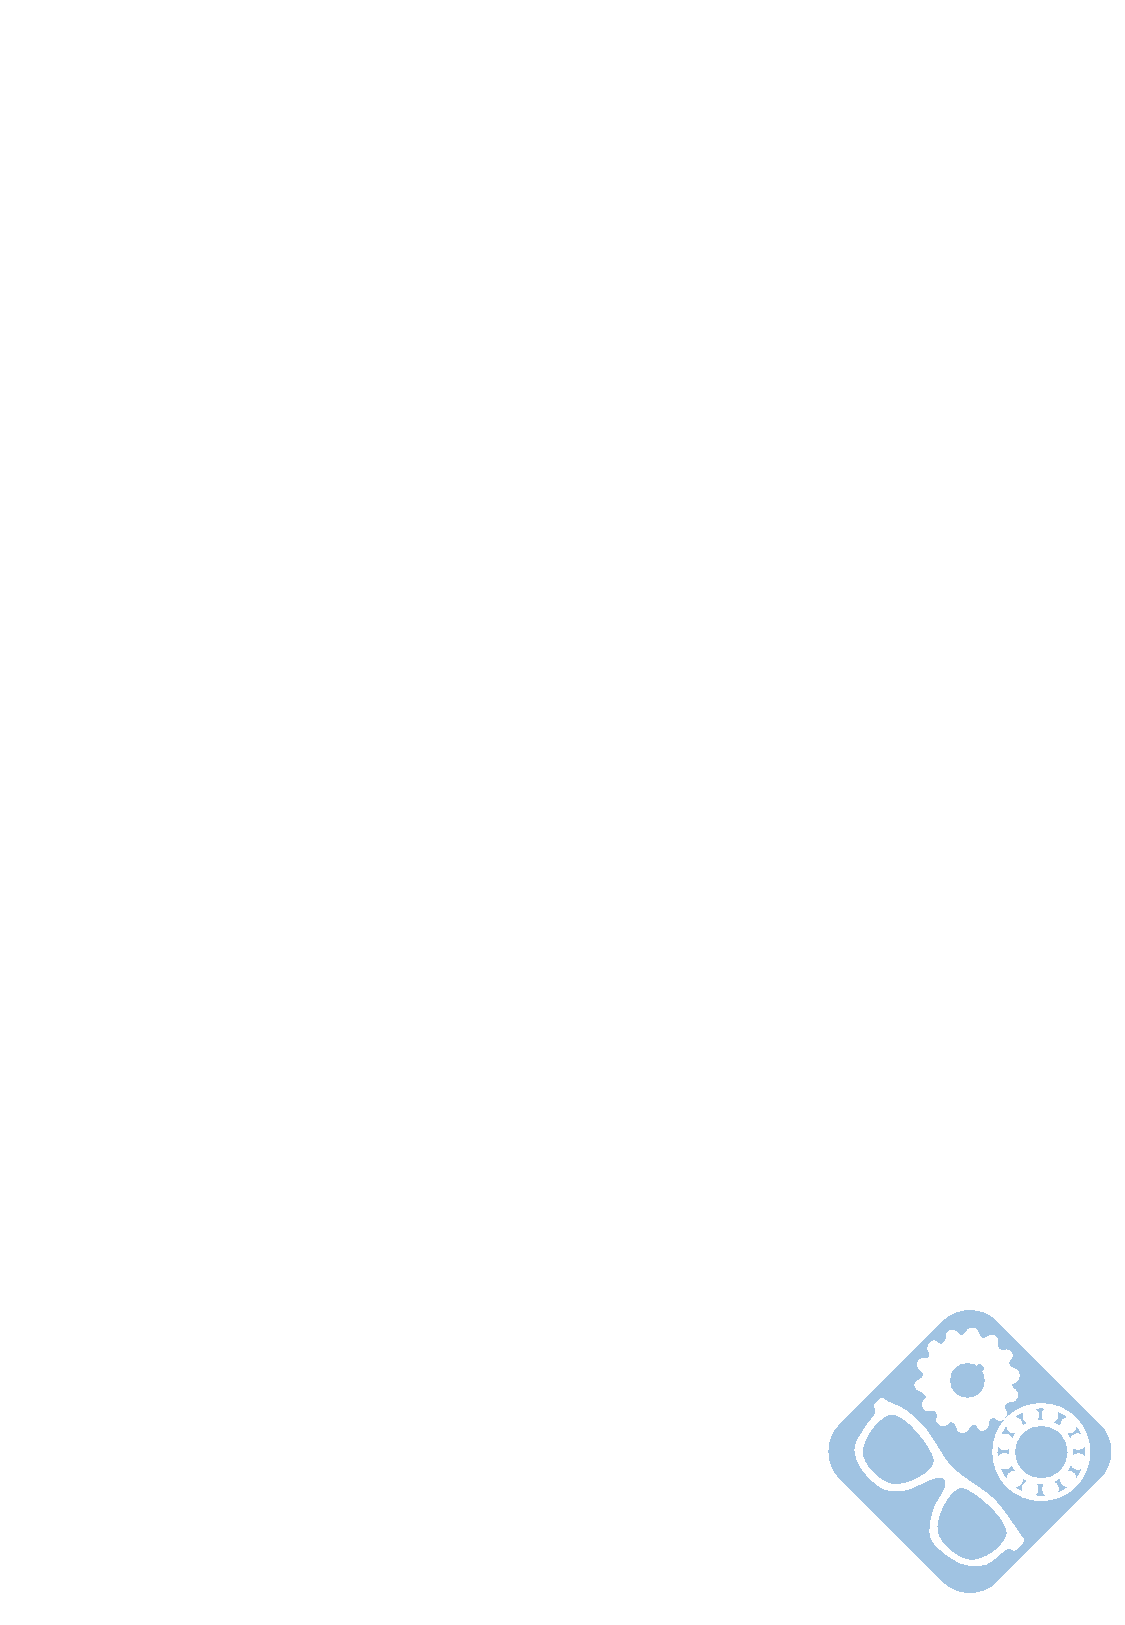
\includegraphics[width=\paperwidth,height=\paperheight,%
keepaspectratio]{../../../img/fond4}%
\end{center}
\vfill
}}}

\begin{document}

\pagestyle{empty}

\AddToShipoutPicture*{\BackgroundPic}


\includegraphics[width=2cm]{../../../img/logo}

\Huge{DS \numero - \sujet}

\vspace{1cm}

\ifdef{\prive}{\begin{center}\colorbox{danger}{\Huge{Avec Correction}}\end{center}}{}

\begin{center}
\centering\huge{PTSI}
\end{center}

\vspace{2cm}


\begin{center}
\centering\Large{\jour}
\end{center}

\vspace{2cm}

\normalsize

\tableofcontents

\newpage

\AddToShipoutPicture{\BackgroundPicdeux}

\pagestyle{fancy}

\begin{center}
\Huge \sujet
\end{center}


\normalsize



Dans l'industrie, il est désormais possible d'associer des tâches robotisées et des tâches manuelles. Après l'essor des robots collaboratifs, Tecdron, entreprise Française basée à La Rochelle, propose une base mobile nommée
TC200, capable de recevoir différents types de bras robotisés - dont des bras collaboratifs - mais aussi de se déplacer de manière autonome dans un environnement industriel complexe composé de robots et d'humains.

Afin de respecter la confidentialité de ce système, les données et résultats présentés dans ce sujet sont approchés et limitatifs par rapport à la solution industrielle réelle.

~\

\begin{wrapfigure}[10]{r}{0.6\textwidth}
	\vspace{-0.8cm}
\begin{center}
 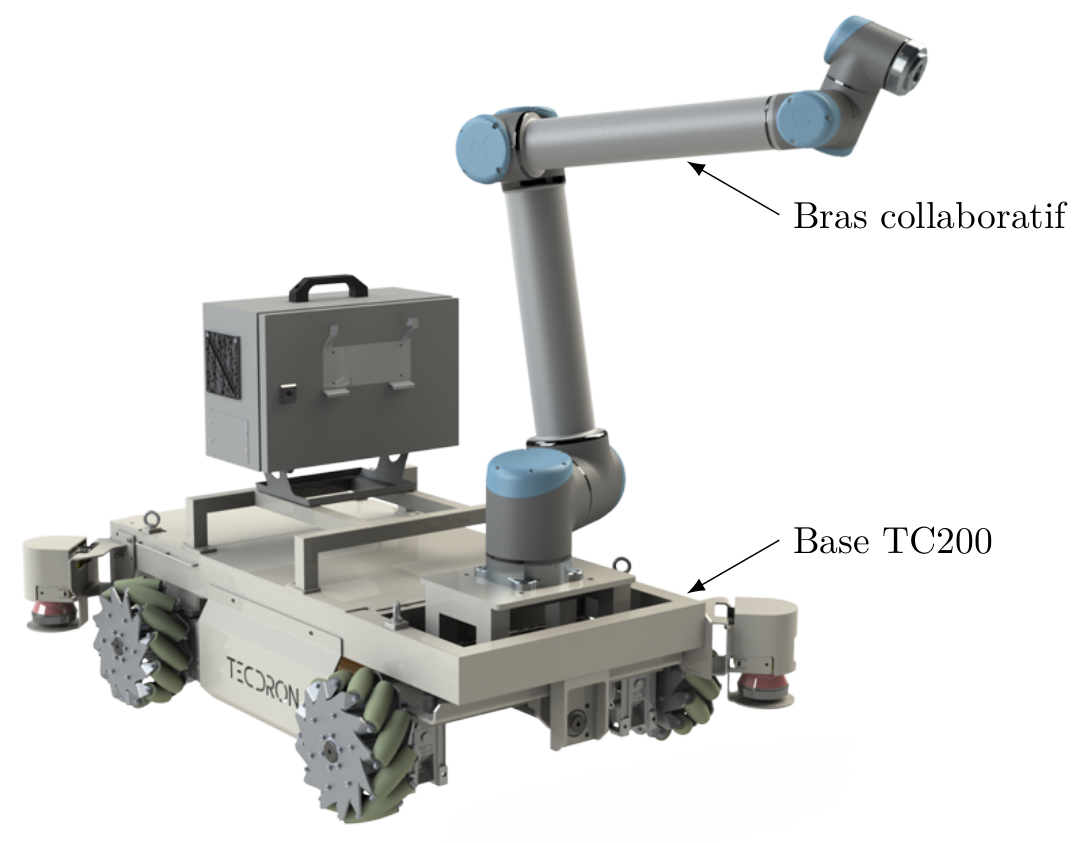
\includegraphics[width=0.6\linewidth]{img/fig01.png}
  \caption{Base TC200 munie d'un bras collaboratif}
\label{fig01}
 \end{center}
\end{wrapfigure}

La base TC200 est utilisée dans le cadre du vissage automatisé de pièces d'avionique dans une carlingue (figure \ref{fig02}).

La base est le support d'un robot de vissage équipé de sa propre commande pour ses mouvements et d'une reconnaissance d'image par caméra afin de bien identifier les emplacements où devront être réalisés les vissages.

\begin{figure}[!ht]
\begin{center}
 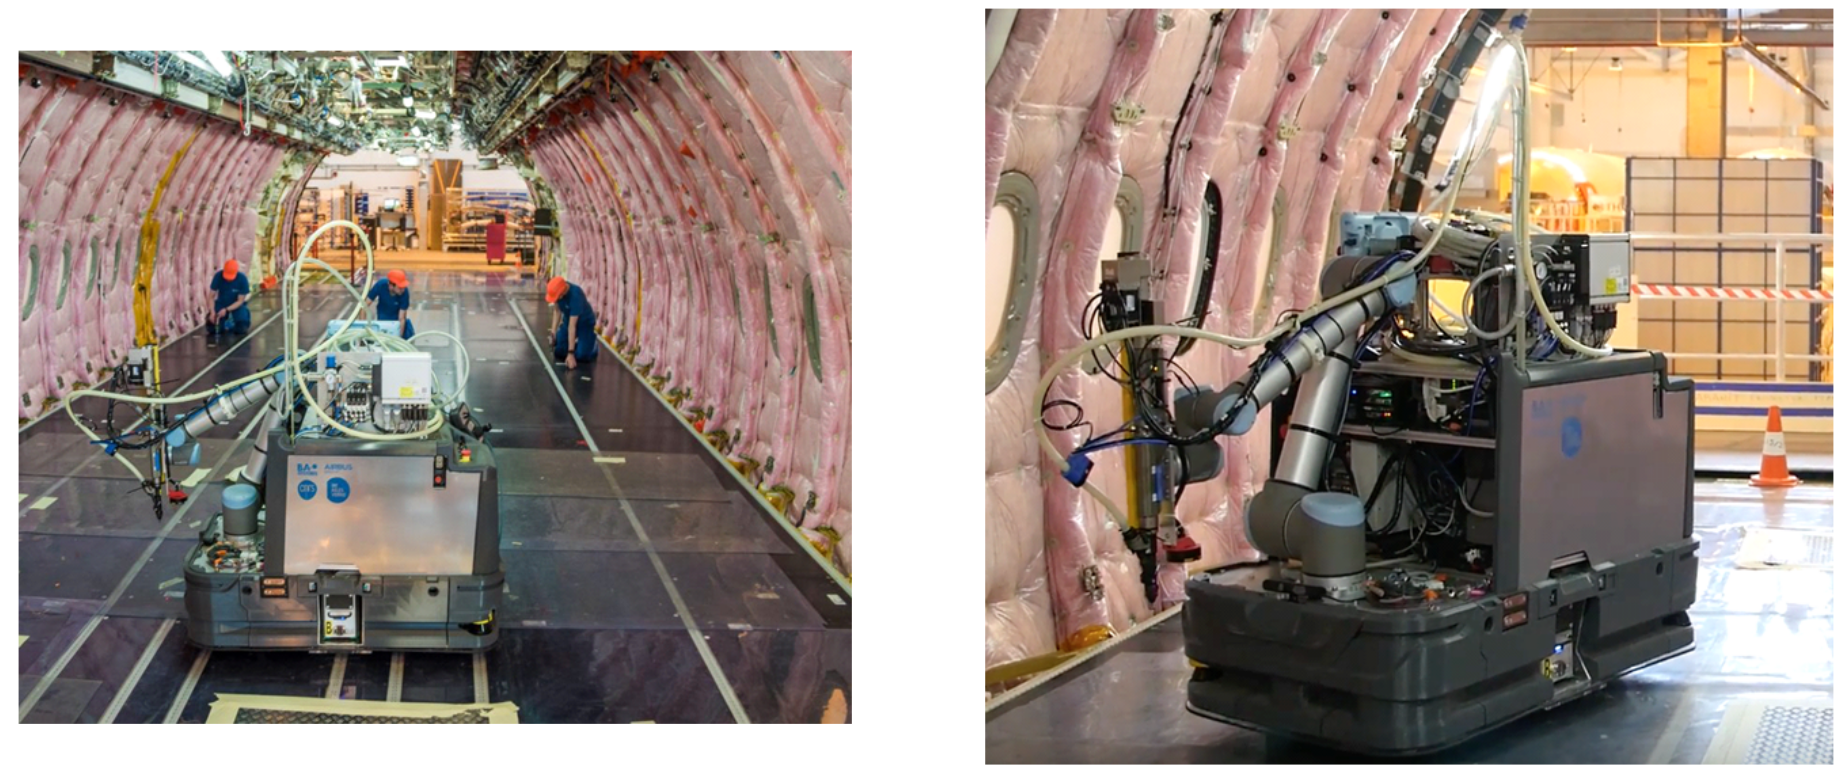
\includegraphics[width=0.8\linewidth]{img/fig02.png}
  \caption{Base TC200 dans l'application de vissage étudiée}
\label{fig02}
 \end{center}
\end{figure}

L'étude proposée dans ce sujet a pour but de valider les solutions technologiques retenues pour permettre à la base TC200 de suivre une trajectoire de consigne définie à l'avance. Elle est découpée en plusieurs parties :
\begin{itemize}
 \item l'analyse et la validation de la structure de la base TC200 pour satisfaire les exigences de mouvements souhaités,
 \item l'étude et la validation des performances des motorisations des roues,
 \item la modélisation dynamique de l'ensemble de la base TC200,
 \item la validation de la commande des motorisations dans le cadre du suivi de trajectoire.
\end{itemize}

\section{Structure de la base TC200}

\paragraph{Objectif} Analyser et valider la structure de la base TC200.

\subsection{Présentation de la base TC200}

La figure \ref{fig03} présente la finalité générale du système et la figure \ref{fig04} ses cas d'utilisation.

\begin{figure}[!ht]
\begin{center}
 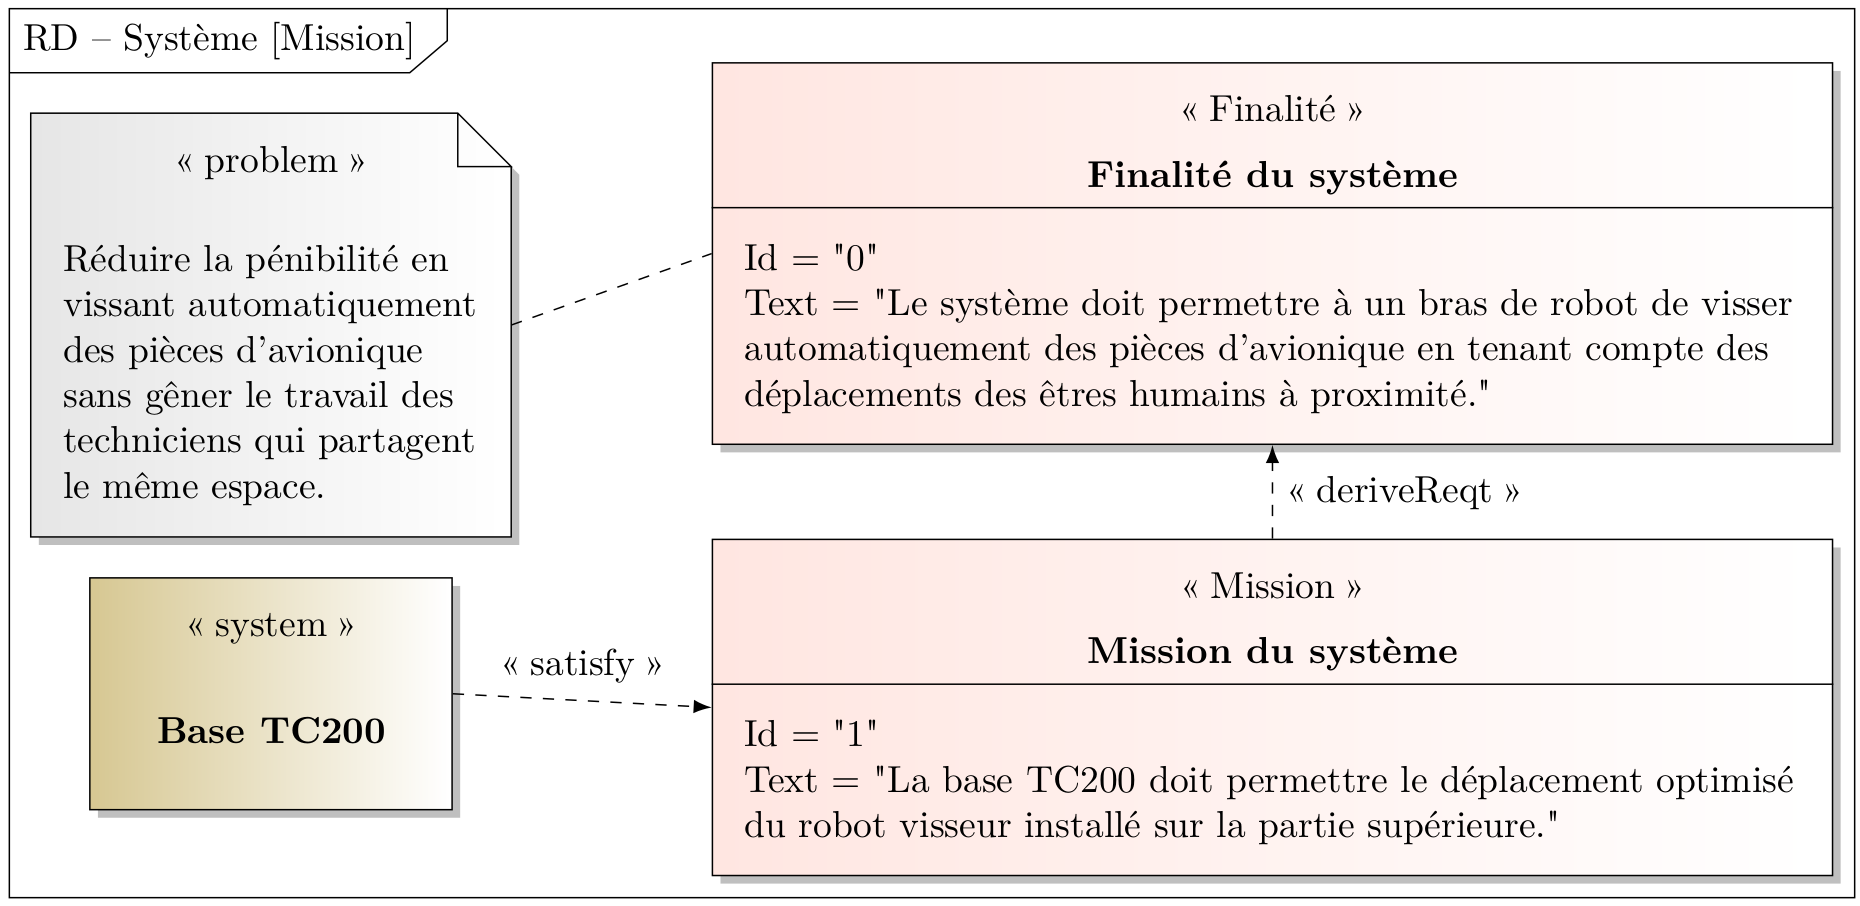
\includegraphics[width=0.9\linewidth]{img/fig03.png}
  \caption{Finalité du système}
\label{fig03}
 \end{center}
\end{figure}

\begin{figure}[!ht]
\begin{center}
 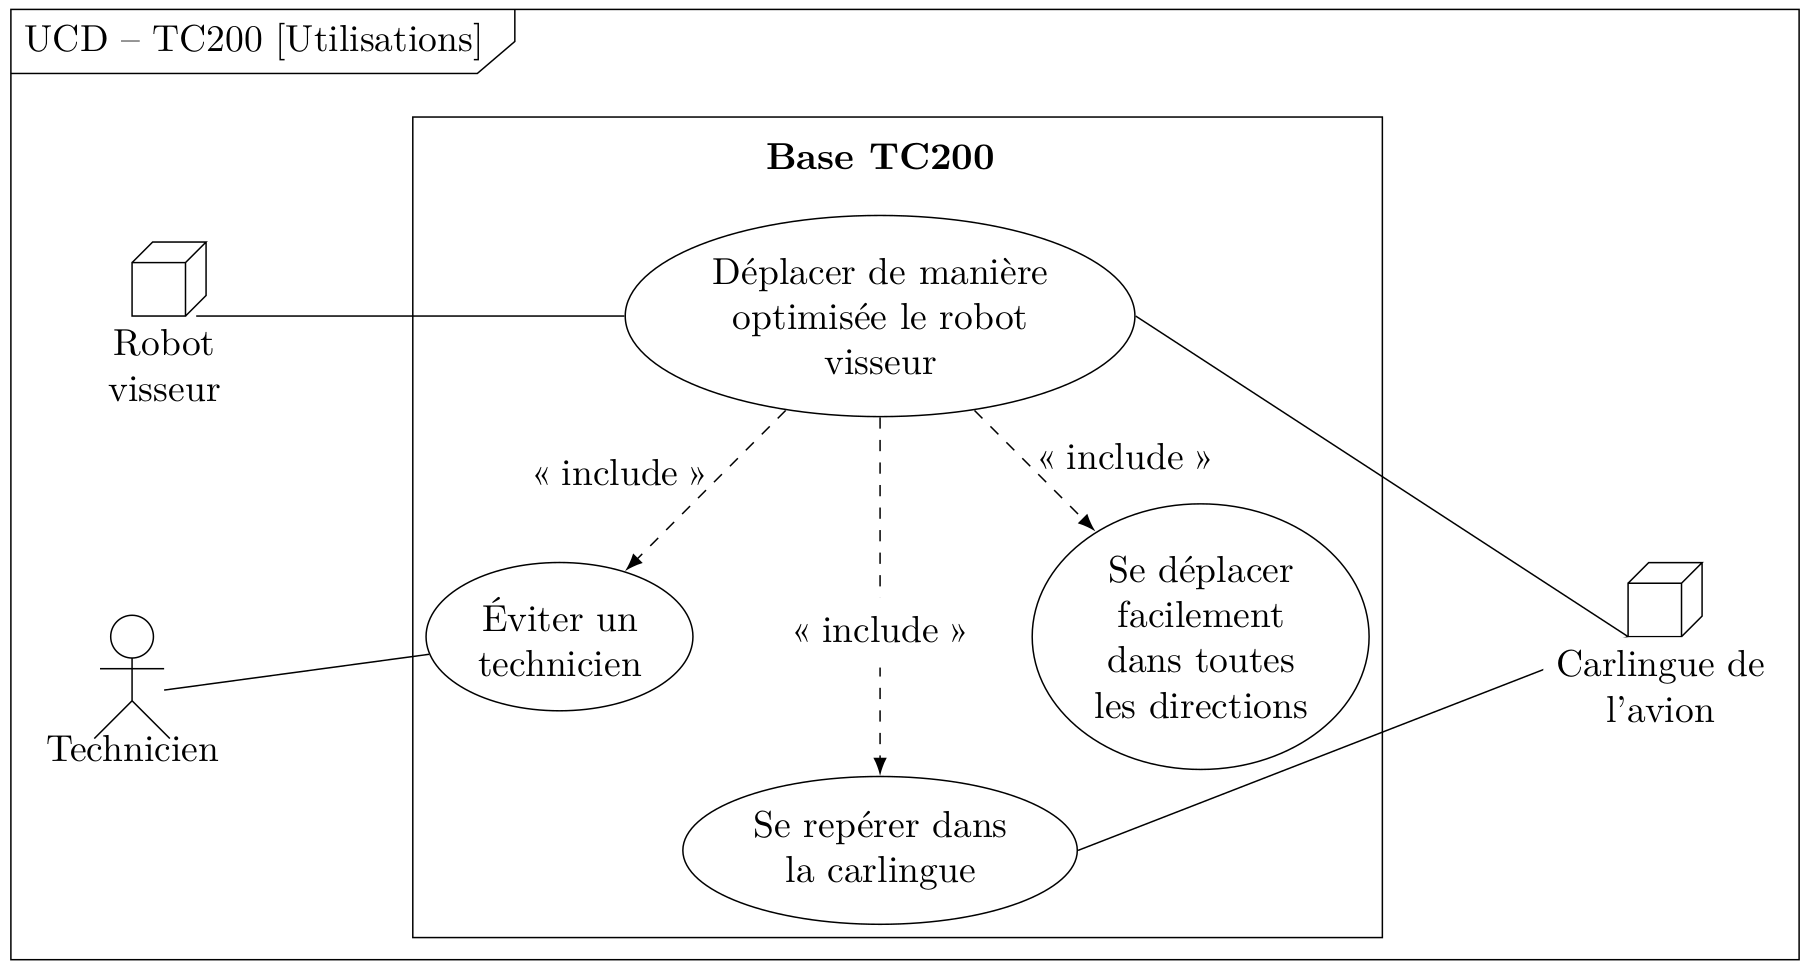
\includegraphics[width=0.9\linewidth]{img/fig04.png}
  \caption{Diagramme des cas d'utilisation du système}
\label{fig04}
 \end{center}
\end{figure}

La base TC200 doit répondre aux exigences de la figure \ref{fig05} qui seront validées tout au long du sujet.

\begin{figure}[!ht]
\begin{center}
 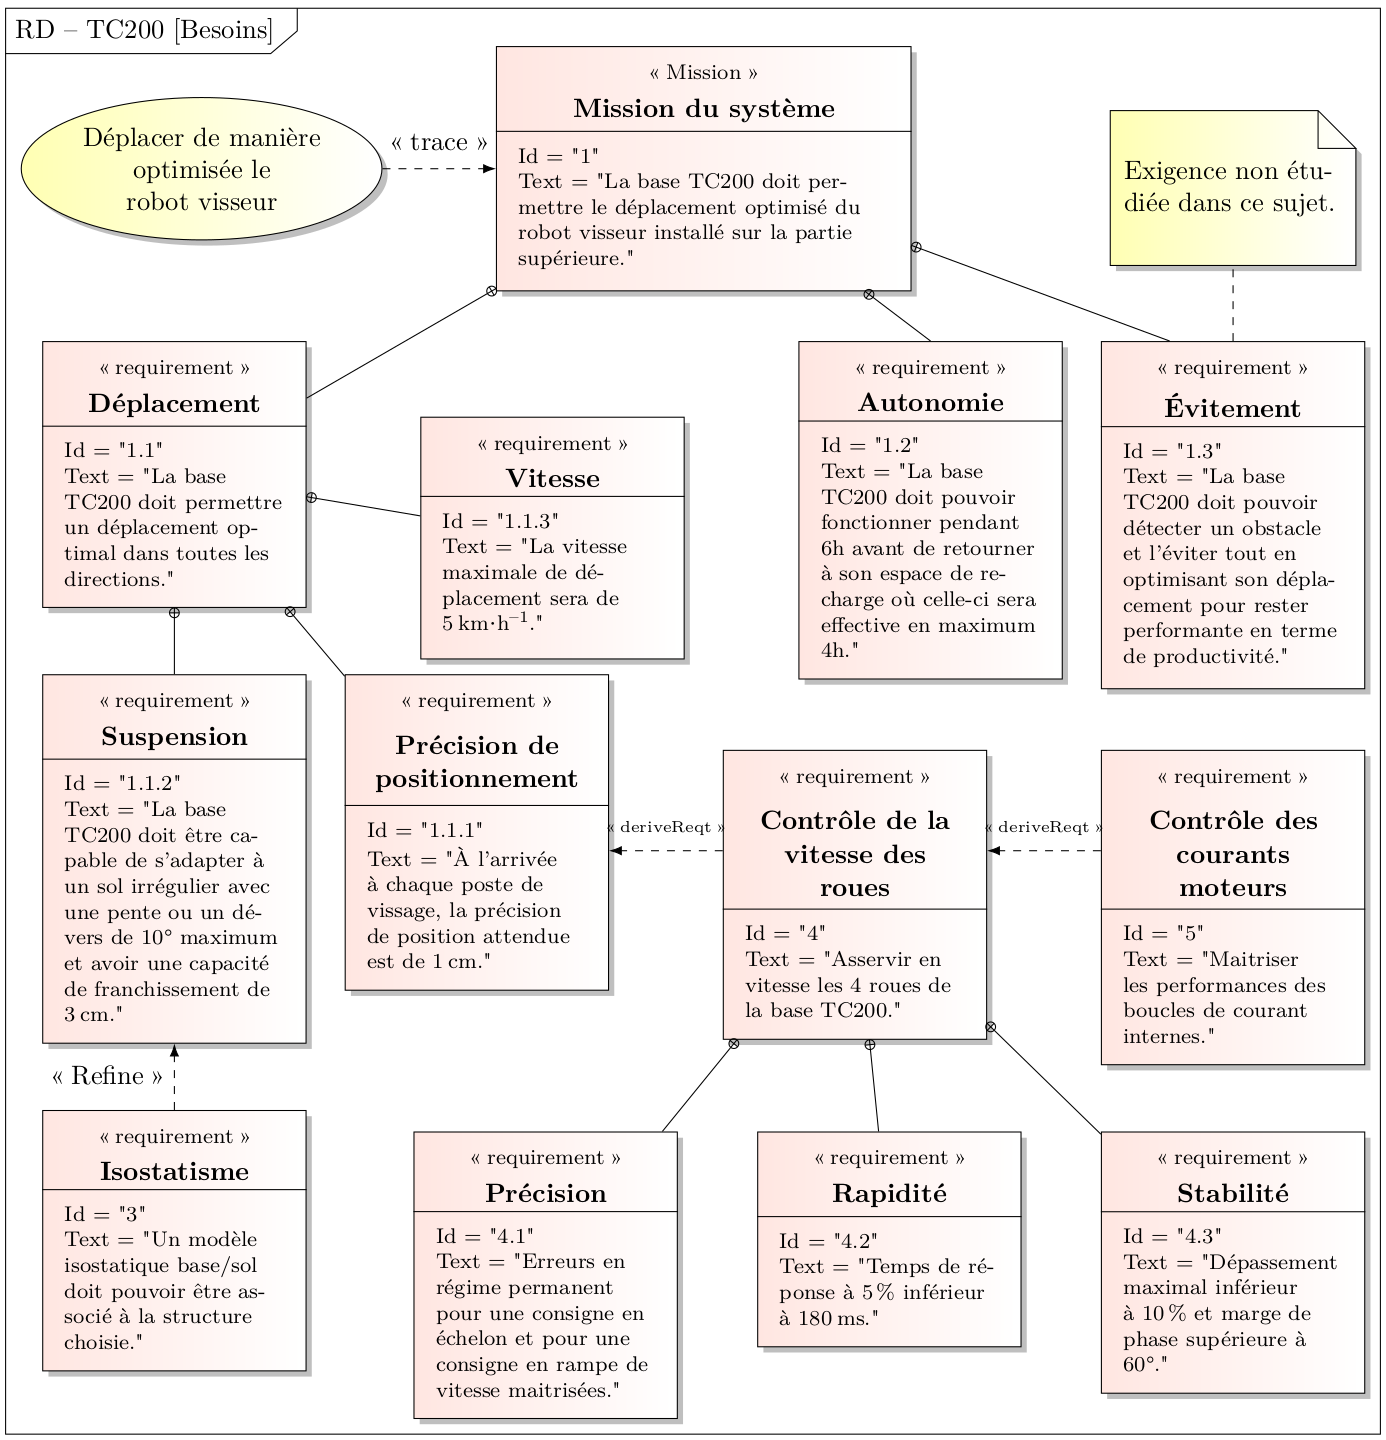
\includegraphics[width=0.9\linewidth]{img/fig05.png}
  \caption{Diagramme des exigences de la base TC200}
\label{fig05}
 \end{center}
\end{figure}

\subsection{Analyse de la solution de déplacement de la base TC200}

\paragraph{Objectif} Analyser le pilotage de la base TC200 pour suivre une trajectoire de consigne.

Le diagramme de définition de blocs de la base TC200 est donné à la figure \ref{fig06}.

\question{À l'aide de la figure \ref{fig06}, compléter le document réponse qui détaille l'organisation structurelle d'une des motorisations.}

~\

Les mouvements possibles de la base TC200 par rapport au sol de la carlingue sont deux translations et une rotation. Chaque roue est équipée de sa propre motorisation. Deux modélisations de la base TC200 sont fournies sur la figure \ref{fig24}, sous la forme de schémas cinématiques. Sur ces modèles, pour chaque roue, seul le rouleau en contact avec le sol est représenté. Toutes les liaisons sont considérées comme parfaites, donc sans jeu et sans adhérence, avec des géométries de contact géométriquement parfaites. Tous les rouleaux représentés sont considérés en contact avec le sol.

\begin{figure}[!ht]
\begin{center}
 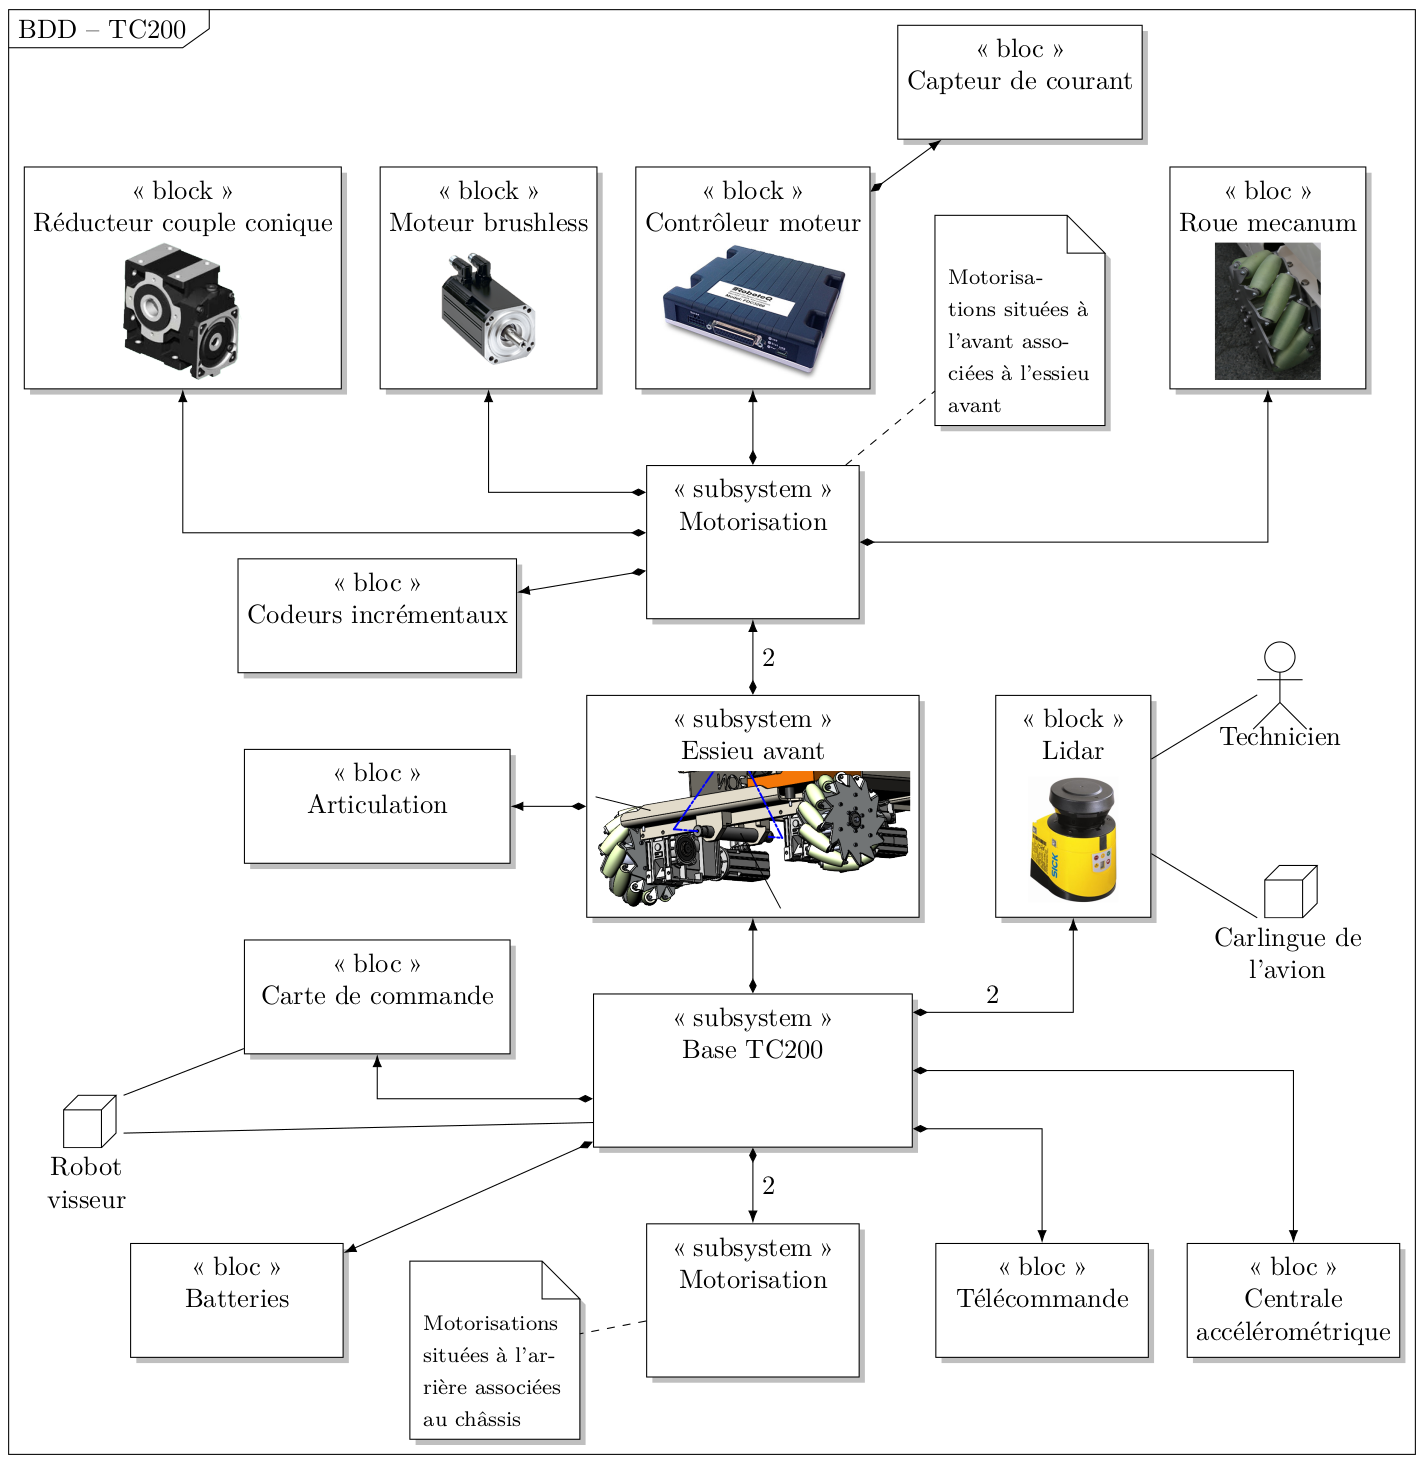
\includegraphics[width=0.9\linewidth]{img/fig06.png}
  \caption{Diagramme de définition de blocs de la base TC200}
\label{fig06}
 \end{center}
\end{figure}

\question{Dans ces hypothèses et en s'appuyant sur des graphes des liaisons, déterminer les degrés d'hyperstatisme des modèles 1 et 2. Justifier la solution adoptée par le constructeur, correspondant au modèle 2, compte
tenu de l'exigence 3.}

~\

Le paramétrage figure dans le tableau \ref{tab01} et les valeurs dimensionnelles dans le tableau \ref{tab02}.

\question{Montrer qu'il est possible à partir de la loi de composition des vitesses $\overrightarrow{V_{I1,11/10}}+\overrightarrow{V_{I1,10/1}}+\overrightarrow{V_{I1,1/0}}=\overrightarrow{0}$ d'obtenir les deux équations scalaires suivantes :}

\begin{center}
\begin{math}
\left\{\begin{array}{l}
V_x-b\omega+r\dot{\beta}_{11}\dfrac{\sqrt{2}}{2}=0\\
V_y+a\omega+(r+R)\omega_{10}+r\dot{\beta}_{11}\dfrac{\sqrt{2}}{2}=0
\end{array}\right.
\end{math}
\end{center}

\newpage

\begin{figure}[!ht]
\begin{center}
 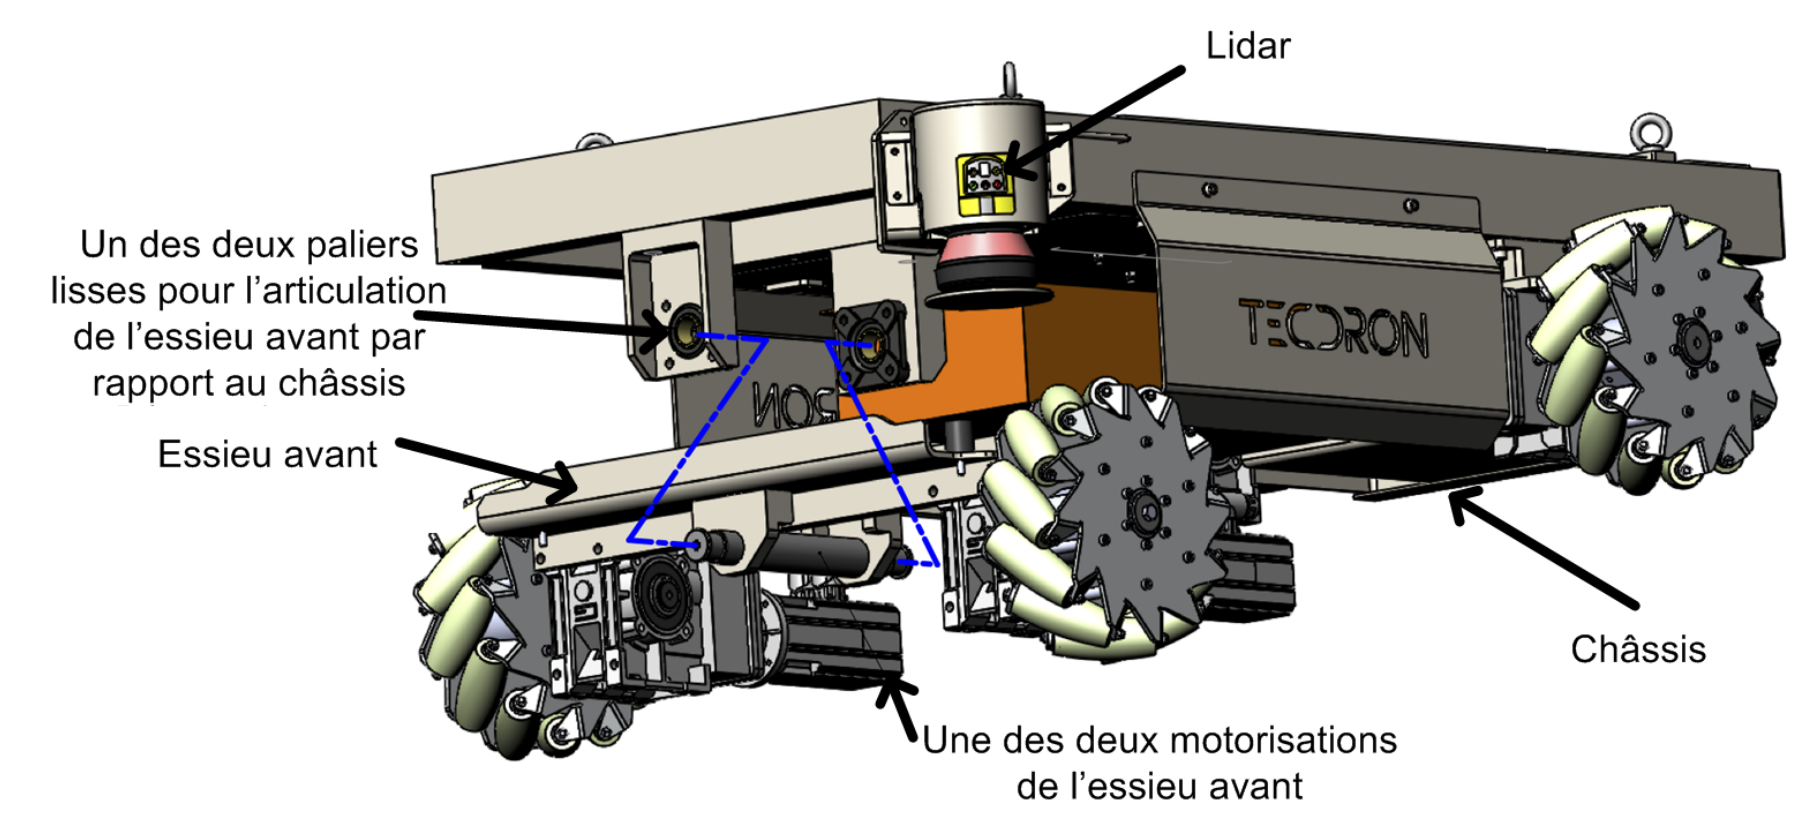
\includegraphics[width=0.8\linewidth]{img/fig07.png}
  \caption{Détails de la base TC200}
\label{fig07}
 \end{center}
\end{figure}

\begin{table}[!ht]
\begin{center}
 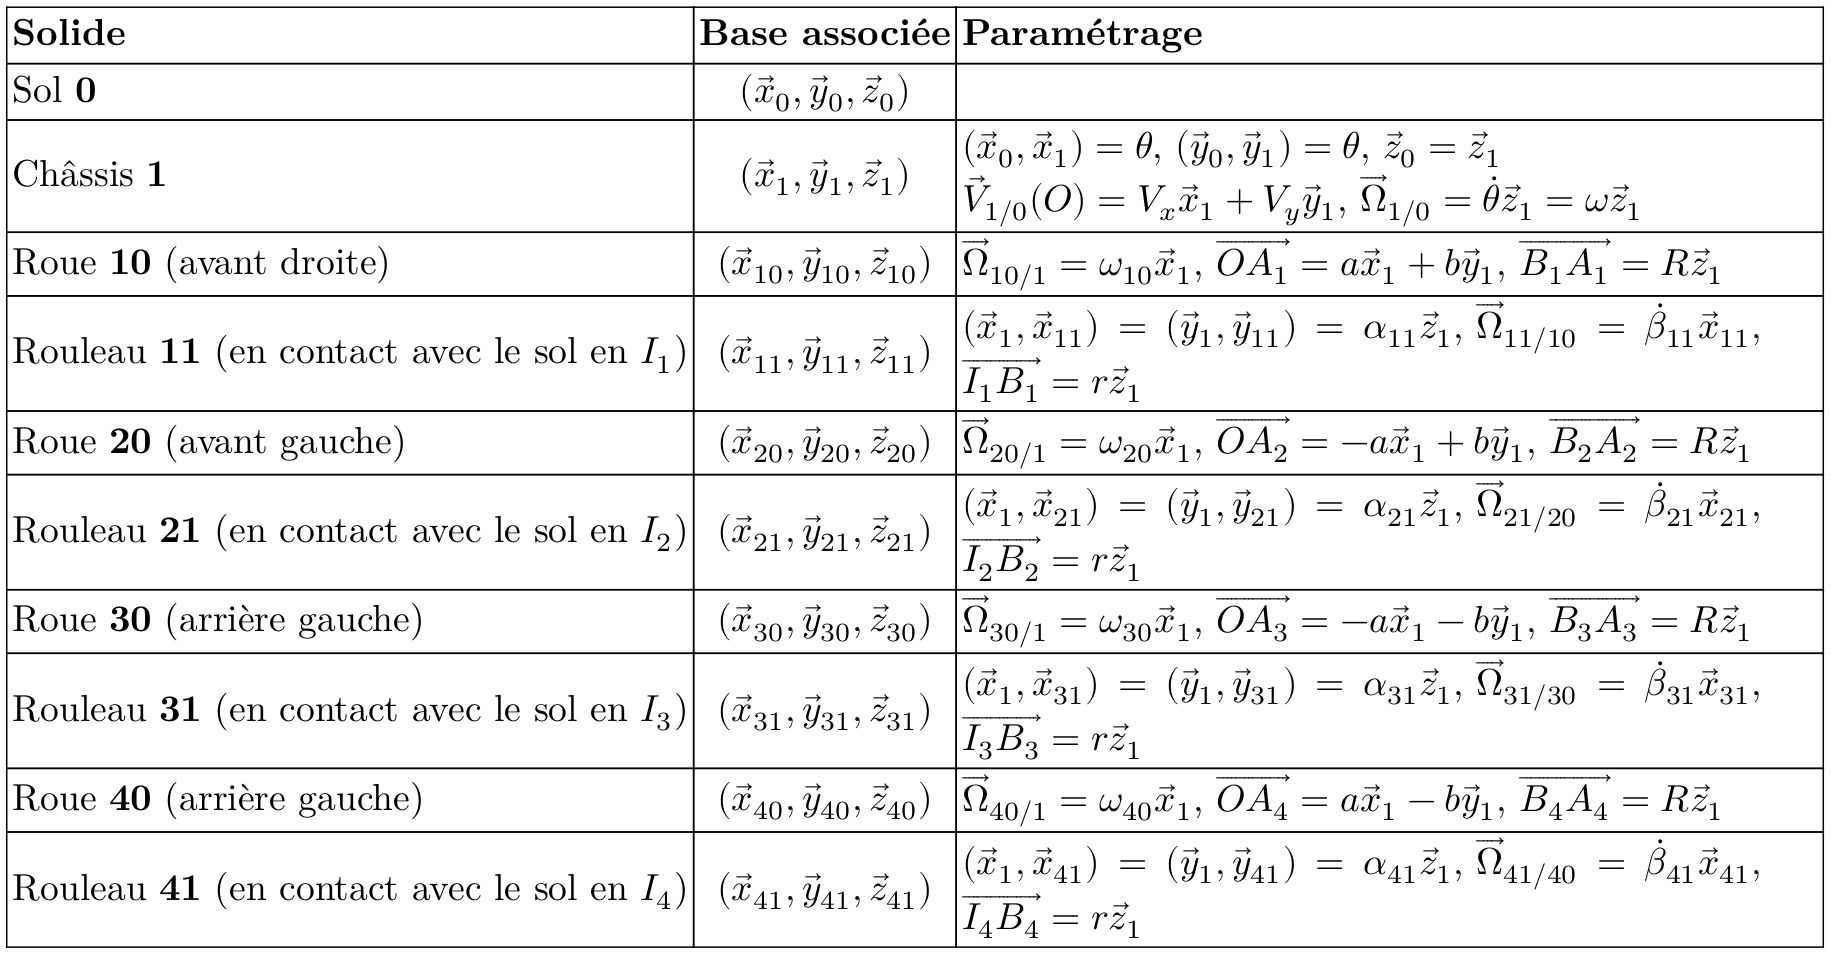
\includegraphics[width=\linewidth]{img/tab01.png}
  \caption{Paramétrage cinématique}
\label{tab01}
\vspace{0.5cm}
 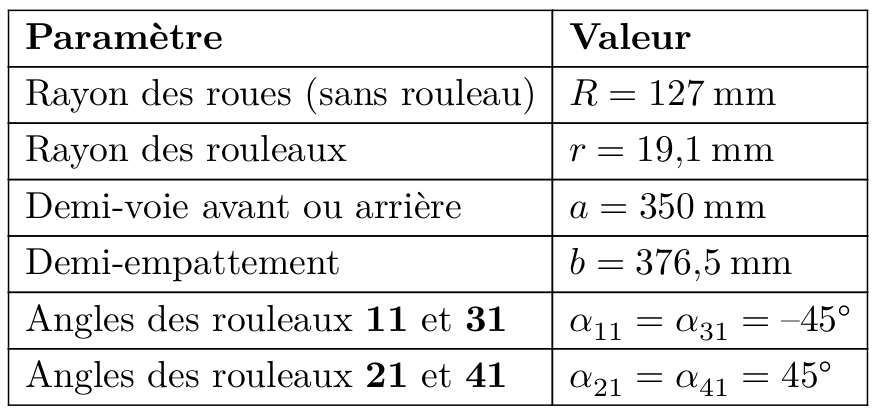
\includegraphics[width=0.5\linewidth]{img/tab02.png}
  \caption{Valeurs dimensionnelles}
\label{tab02}
 \end{center}
\end{table}

\newpage

Par des relations de même type, il est possible d'ajouter les six équations scalaires suivantes:

\begin{center}
\begin{math}
\left\{\begin{array}{l}
V_x-b\omega-r\dot{\beta}_{21}\dfrac{\sqrt{2}}{2}=0\\
V_y-a\omega+(r+R)\omega_{20}+r\dot{\beta}_{21}\dfrac{\sqrt{2}}{2}=0
\end{array}\right.
\end{math}

\begin{math}
\left\{\begin{array}{l}
V_x+b\omega+r\dot{\beta}_{31}\dfrac{\sqrt{2}}{2}=0\\
V_y-a\omega+(r+R)\omega_{30}+r\dot{\beta}_{31}\dfrac{\sqrt{2}}{2}=0
\end{array}\right.
\end{math}

\begin{math}
\left\{\begin{array}{l}
V_x+b\omega-r\dot{\beta}_{41}\dfrac{\sqrt{2}}{2}=0\\
V_y+a\omega+(r+R)\omega_{40}+r\dot{\beta}_{41}\dfrac{\sqrt{2}}{2}=0
\end{array}\right.
\end{math}
\end{center}

Les paramètres cinématiques du châssis par rapport au sol sont notés sous la forme d'une matrice colonne $V$ et l'ensemble des vitesses angulaires des roues par rapport au châssis sous la forme d'une matrice colonne $W$ définies par:

\begin{center}
$V=\left(\begin{array}{c}
\omega \\ V_x \\ V_y
\end{array}\right)$ et $W=\left(\begin{array}{c}
\omega_{10} \\ \omega_{20} \\ \omega_{30} \\ \omega_{40}
\end{array}\right)$
\end{center}

\question{Déterminer la matrice $M$ telle que $W=M\cdot V$.}

~\

La vitesse standard de la base TC200 est de $1m\cdot s^{-1}$, inférieure à la vitesse maximale des exigences de $5km\cdot h^{-1}$.

\question{Déterminer $W_1$, $W_2$ et $W_3$ correspondant respectivement à des paramètres de mouvements de la base définis par $V_1=\left(\begin{array}{c}
0 \\ 0 \\ 1 \end{array}\right)$, $V_2=\left(\begin{array}{c}
0 \\ 1 \\ 0 \end{array}\right)$  et $V_3=\left(\begin{array}{c}
0 \\ 1 \\ 1 \end{array}\right)$ (c'est à dire $W_1=M\cdot V_1$,...).

Connaissant $W$, expliquer s'il est possible de déterminer de manière unique $V$. Commenter ce résultat vis-à-vis de l'exigence 3.}

~\

Pour la suite du sujet, le mouvement étudié se limite à une translation de la base TC200. Les vitesses de rotation de consigne des roues par rapport au châssis s'expriment alors plus simplement en fonction des paramètres du
mouvement sous la forme:

\begin{center}
\begin{eqnarray}
\omega_{10}(t)=\omega_{30}(t)=\frac{V_x(t)-V_y(t)}{r+R} \label{eq1} \\
\omega_{20}(t)=\omega_{40}(t)=-\frac{V_x(t)+V_y(t)}{r+R} \label{eq2}
\end{eqnarray}
\end{center}

Dans cette partie, l'asservissement de vitesse des actionneurs est considéré comme parfait, c'est-à-dire que les vitesses réelles sont égales aux vitesses de consigne.

La figure \ref{fig08} propose un graphe d'états pour la commande des vitesses de rotation des roues du robot. Dans ce graphe d'états, la variable $e$ est une variable interne.

\newpage

\begin{figure}[!ht]
\begin{center}
 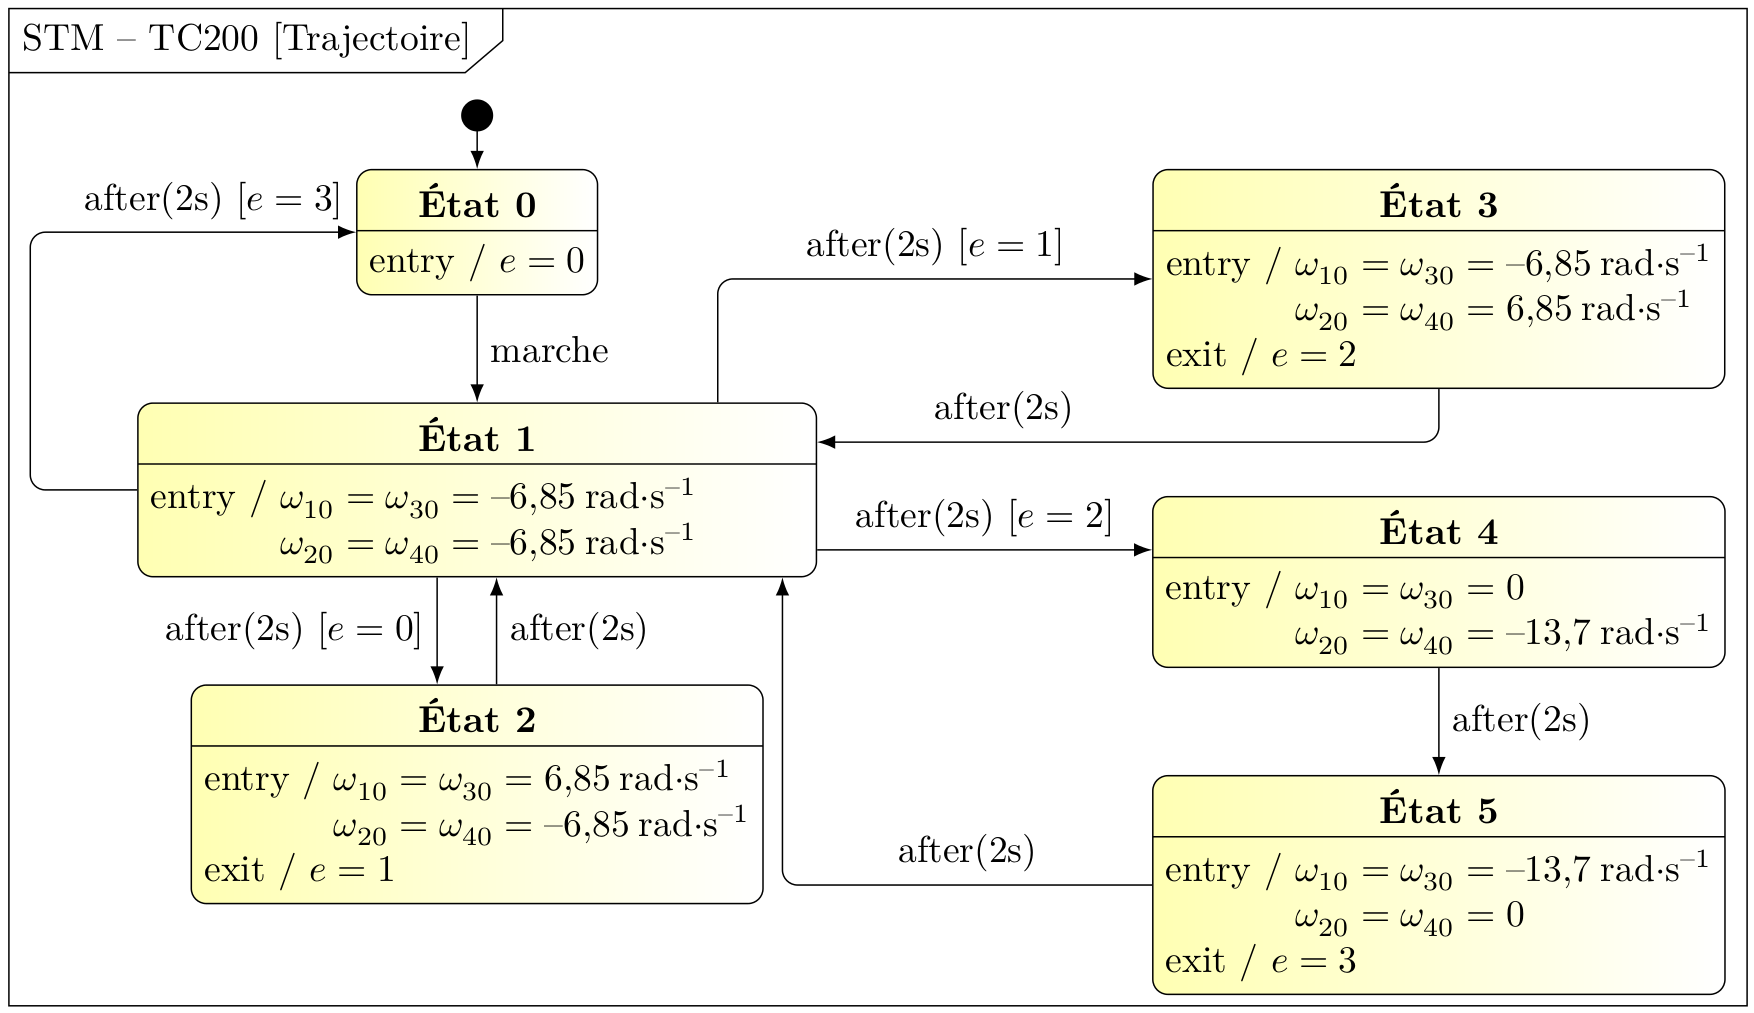
\includegraphics[width=0.9\linewidth]{img/fig08.png}
  \caption{Graphe d'états des mouvements de la base TC200}
\label{fig08}
 \end{center}
\end{figure}

\vspace{-1cm}

\question{Tracer sur le document réponse, la trajectoire du point $O$ de la base TC200 correspondant à ce graphe d'états, après appui sur le bouton marche et en s'appuyant sur les relations \ref{eq1} et \ref{eq2}.}

~\

C'est la qualité de l'asservissement de vitesse des motorisations étudié dans les parties suivantes qui permet de suivre correctement cette trajectoire de consigne.

Le modèle 2 précédent nécessite le recours à une articulation de type pivot, de l'essieu avant par rapport au châssis, qui doit résister aux contraintes mécaniques.

\subsection{Validation du dimensionnement de l'articulation de l'essieu avant}

\paragraph{Objectif} Valider le dimensionnement de l'axe de l'articulation de l'essieu avant par rapport au châssis.

Une modélisation de type poutre est proposée pour l'axe de l'articulation entre l'essieu avant et le châssis sur la figure \ref{fig09}. Le paramétrage spécifique utilisé dans cette figure est indépendant du paramétrage utilisé dans tout le reste du sujet.

\begin{figure}[!ht]
\begin{center}
 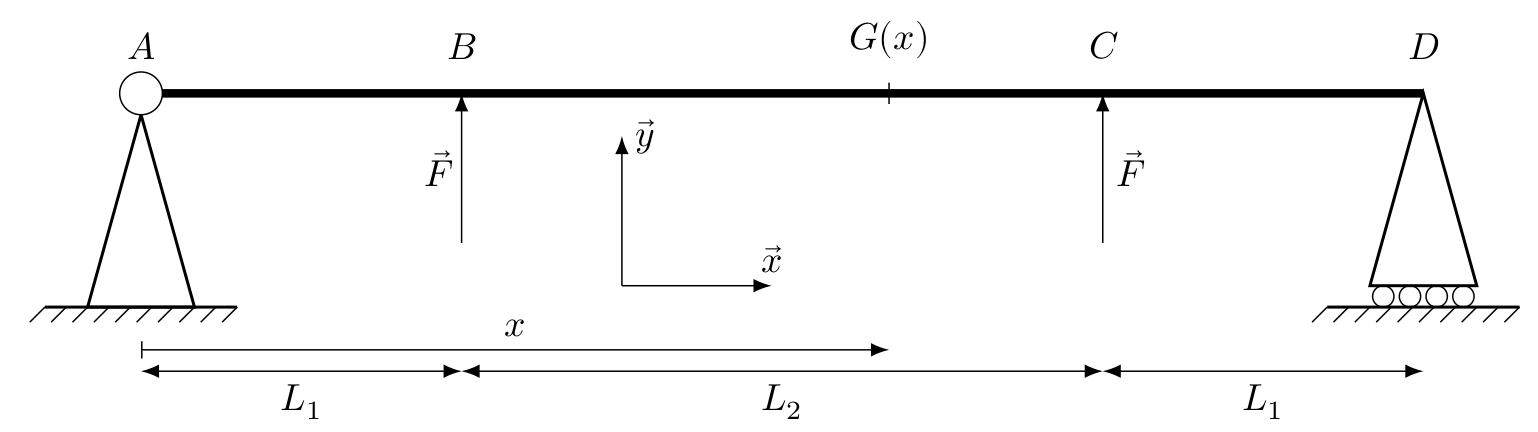
\includegraphics[width=0.7\linewidth]{img/fig09.png}
  \caption{Modélisation spécifique à la validation du dimensionnement de l'articulation essieu/châssis}
\label{fig09}
 \end{center}
\end{figure}

\vspace{-0.5cm}

Les deux actions mécaniques exercées par l'essieu avant sur l'axe sont modélisées par les deux torseurs d'actions mécaniques
$\left\{\begin{array}{c} F\vec{y}\\ 0 \end{array} \right\}_B$ et $\left\{\begin{array}{c} F\vec{y}\\ 0 \end{array} \right\}_C$ avec F = 500 N. L'action mécanique associée à la pesanteur n'est pas prise en compte. La liaison en A sera modélisée par une pivot d'axe ($A,\vec{z}$) et celle en D par une ponctuelle de normale ($D,\vec{y}$). L'exigence attendue pour cette articulation est détaillée dans le tableau \ref{tab03}.

L'axe est un cylindre en acier de diamètre $d = 15 mm$, modélisé par une poutre droite (figure \ref{fig09}). Les hypothèses de Navier-Bernoulli sont considérées vérifiées.

Le moment quadratique de l'axe cylindrique est $I_{G,\vec{z}}=\dfrac{\pi d^4}{64}$. Les dimensions sont $L_1 = 50 mm$ et $L_2 = 150 mm$.

\question{Déterminer les actions mécaniques exercées par les appuis sur la poutre aux points A et D.}

~\

Une étude de flexion a permis de déterminer la valeur de la flexion dans la poutre:
\begin{itemize}
 \item $M_{fz}(x)=-F\cdot x$ pour $G\in[AB]$ ($0\leq x\leq L_1$), 
 \item $M_{fz}(x)=-F\cdot L_1$ pour $G\in[BC]$ ($L_1\leq x\leq L_1+L_2$),
 \item $M_{fz}(x)=-F\cdot (x-2L_1-L_2)$ pour $G\in[CD]$ ($L_1+L_2\leq x\leq 2L_1+L_2$).
\end{itemize}

\begin{table}[!ht]
\begin{center}
 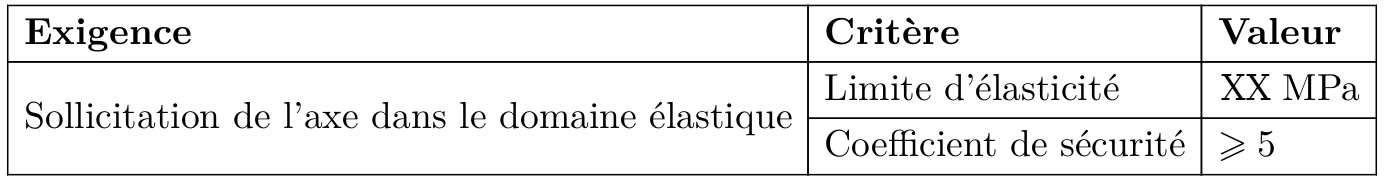
\includegraphics[width=0.8\linewidth]{img/tab03.png}
 \end{center}
  \caption{Exigence associée à la résistance mécanique de l'articulation de l'essieu avant}
\label{tab03}
\end{table}

Un essai de traction réalisé sur le matériau de l'axe est présenté à la figure \ref{fig10}.

\begin{figure}[!ht]
\begin{center}
 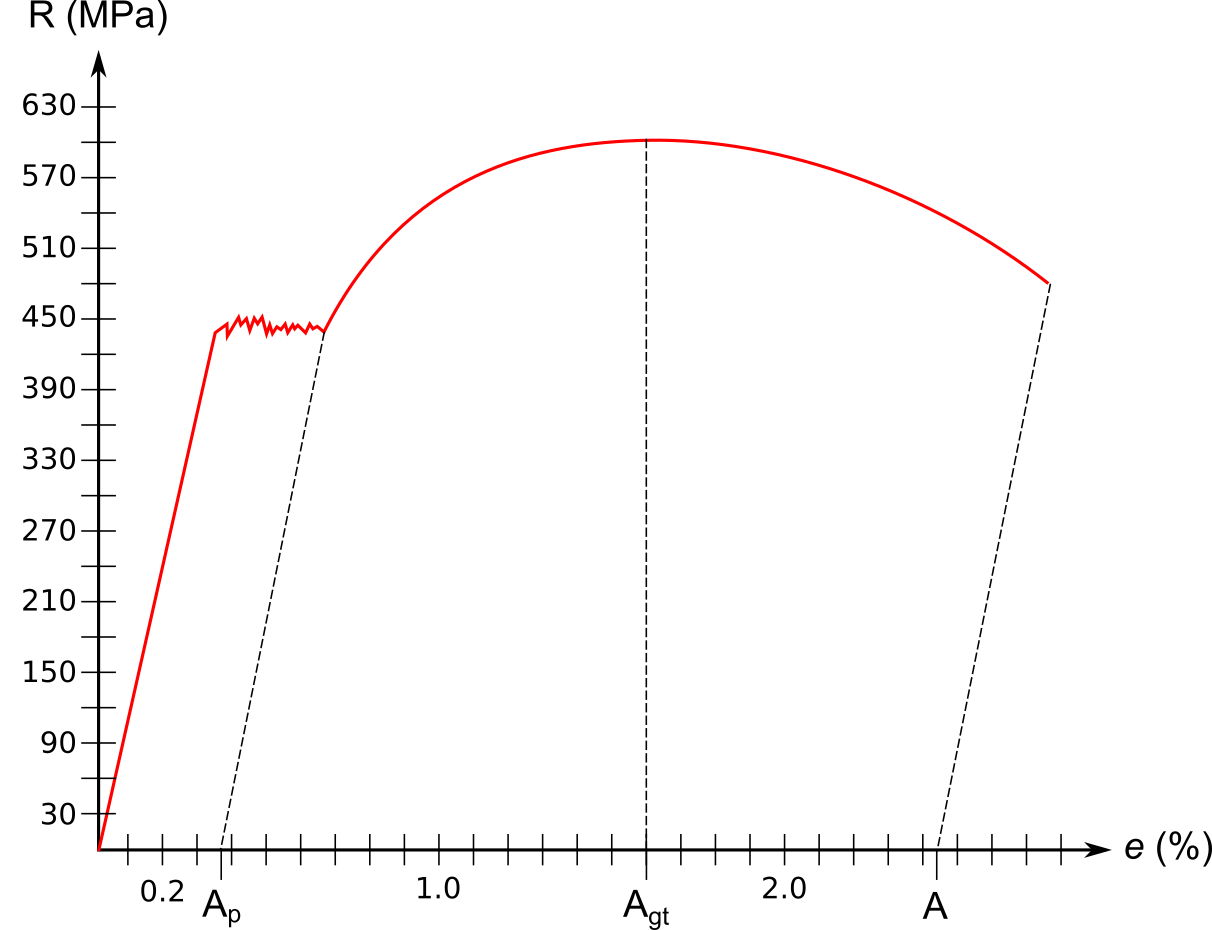
\includegraphics[width=0.5\linewidth]{img/fig10.png}
 \end{center}
  \caption{Essai de traction de l'acier de l'axe}
\label{fig10}
\end{figure}

\question{Déterminer sur l'essai de traction présenté, les valeurs de $R_e$, $R_m$ et $A\%$.}

L'expression de la contrainte normale $\sigma(x,y)$ en fonction de la distance $y$ par rapport à la ligne neutre est donnée par la relation $\sigma(x,y)=-\dfrac{M_{fz}(x)}{I_{G,\vec{z}}}y$ pour une section située à l'abscisse $x$.

\question{Pour la section la plus sollicitée ($|M_{fz}(x)|$ maximum), déterminer l'expression de la contrainte maximale et faire l'application numérique pour $y=\dfrac{d}{2}$.}

\question{Conclure sur le respect des exigences du tableau \ref{tab03}.}

\section{Motorisation de la base TC200}

\subsection{Validation des machines et des contrôleurs}

Afin de déplacer la base TC200, il faut contrôler les vitesses ainsi que les couples de chacune des machines conformément à la commande de la figure \ref{fig12}, qui montre la structure de l'asservissement d'une des machines,
qui est la même pour toutes les chaînes de motorisation. Cet asservissement nécessite une boucle interne de courant (en fait des 3 courants des enroulements de la machine) pour maîtriser également le couple.

\begin{figure}[!ht]
\begin{center}
 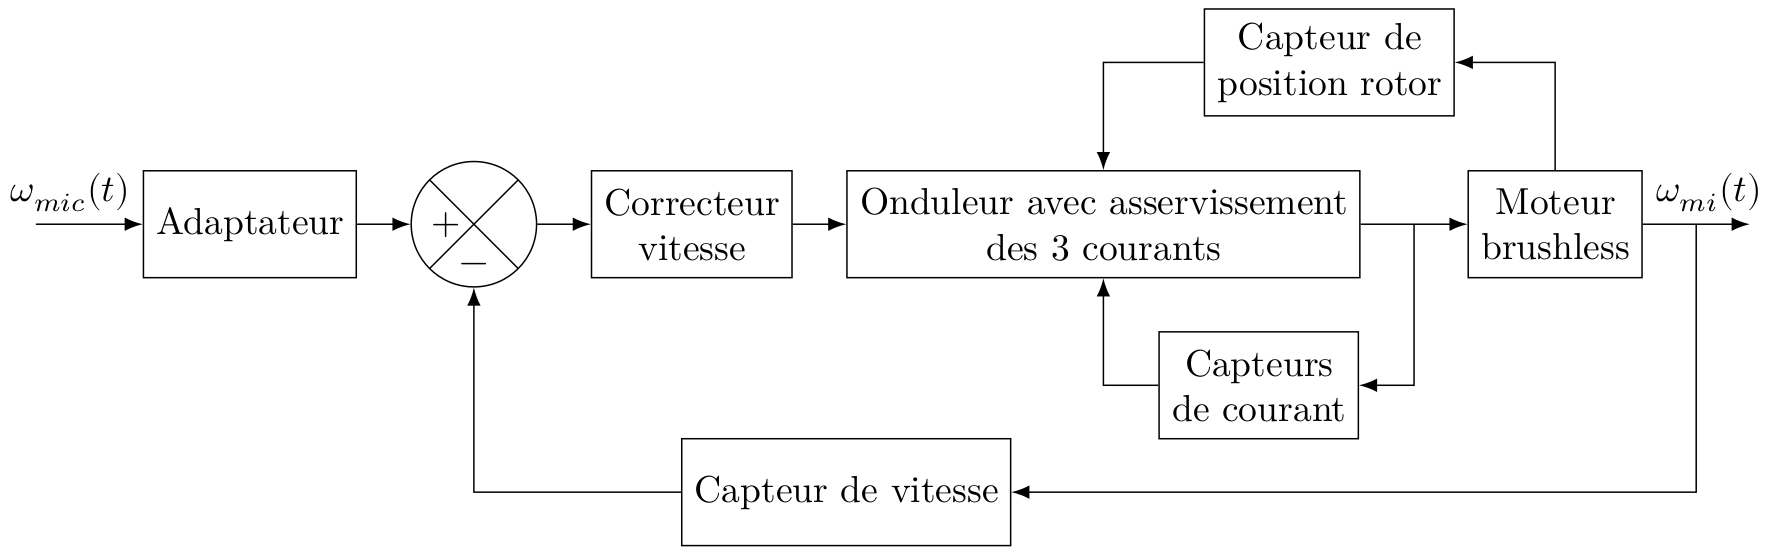
\includegraphics[width=0.8\linewidth]{img/fig12.png}
 \end{center}
  \caption{Structure de l'asservissement d'une des motorisations}
\label{fig12}
\end{figure}

\vspace{-0.5cm}

\question{Donner la définition d'un onduleur.}

\subsection{Étude de la boucle de courant}

\paragraph{Objectif} Valider les performances de la boucle de courant.

C'est le contrôle du couple instantané $C_{em}(t)$ de chaque moteur qui permet de contrôler la vitesse, y compris en régime transitoire. Ce contrôle est délicat puisqu'il dépend des courants instantanés des trois phases et de
la position du rotor obtenue par le traitement des signaux issus des codeurs incrémentaux. Une commande plus rapide et plus efficace consiste à travailler dans un système diphasé fictif équivalent grâce à un modèle mathématique adapté (transformation de Park) dans le plan \og dq \fg (d pour direct et q pour quadrature).

Le courant $i_d(t)$ est asservi à une valeur nulle. Les équations obtenues sont:

\begin{center}
\begin{eqnarray}
V_q(t)=R_{eq}i_q(t)+L_{eq}\dfrac{\d i_q(t)}{\d t}+K_e\omega_m(t) \label{eq3}\\
C_{em}(t)=K_ti_q(t)=C_f(t)+J_{eq}\dfrac{\d\omega_m(t)}{\d t} \label{eq4}
\end{eqnarray}
\end{center}

\begin{tabular}{l l l}
$L_{eq}$ & ($H$) & inductance équivalente d'induit sur l'axe d supposée égale à celle sur l'axe q \\
$R_{eq}$ & ($\Omega$) & résistance équivalente d'enroulement statorique \\
$J_{eq}$ & ($kg\cdot m^2$) & inertie équivalente ramenée au rotor moteur \\
$\omega_m(t)$ & ($rad\cdot s^{-1}$) & vitesse de rotation du rotor \\
$C_f(t)$ & ($N\cdot m$) & couple de frottement \\
$C_{em}(t)$  & ($N\cdot m$) & couple électromagnétique supposé égal au couple moteur \\
$K_e$ & ($V\cdot s\cdot rad^{-1}$) & constante de force électromotrice \\
$K_t$ & ($N\cdot m\cdot A^{-1}$) & constante de couple \\
$V_q (t)$ & $(V)$ & tension d'alimentation de la phase fictive en quadrature.
\end{tabular}

~\

Le schéma de principe de l'asservissement de courant est représenté figure \ref{fig13}.

\begin{figure}[!ht]
\begin{center}
 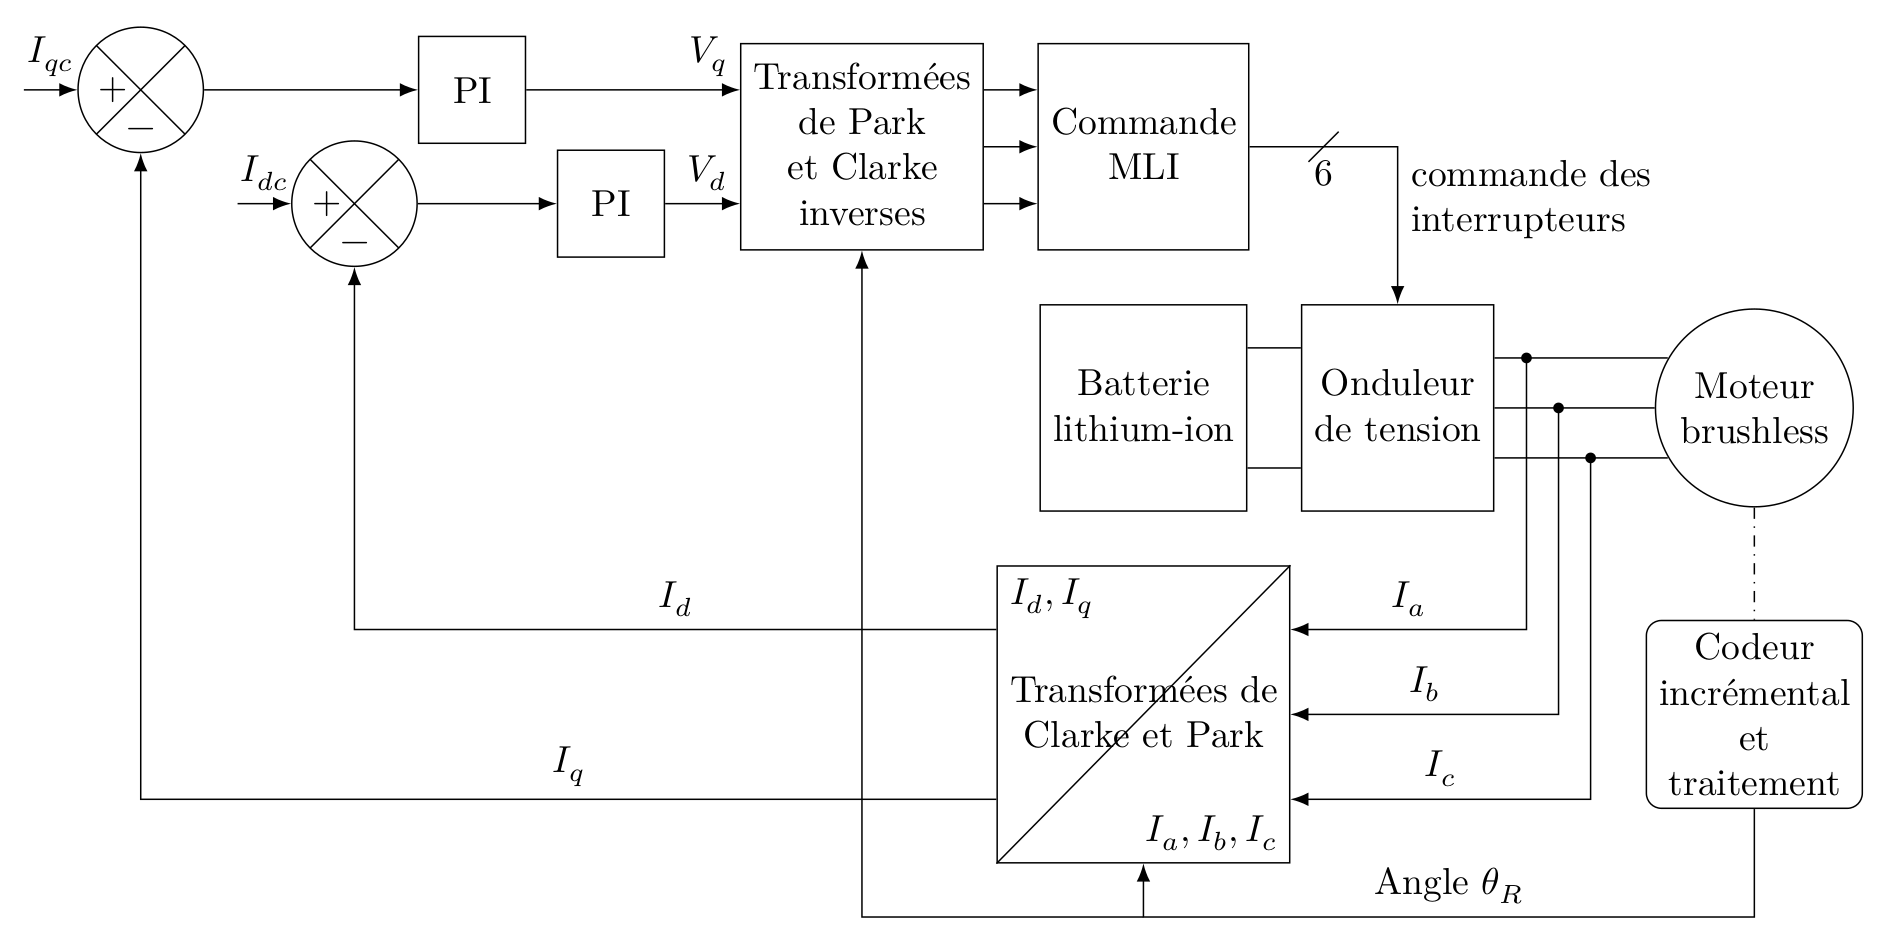
\includegraphics[width=0.8\linewidth]{img/fig13.png}
 \end{center}
  \caption{Principe de l'asservissement de courant}
\label{fig13}
\end{figure}

Le courant $i_d(t)$ est parfaitement asservi à la valeur $i_{dc}(t)=0$ pour la suite, ce qui permet de s'intéresser uniquement à l'asservissement du courant $i_q(t)$.

Avec des hypothèses simplificatrices, les boucles d'asservissement peuvent être formalisées au moyen de techniques classiques développées pour les systèmes linéaires.

\begin{figure}[!ht]
\begin{center}
 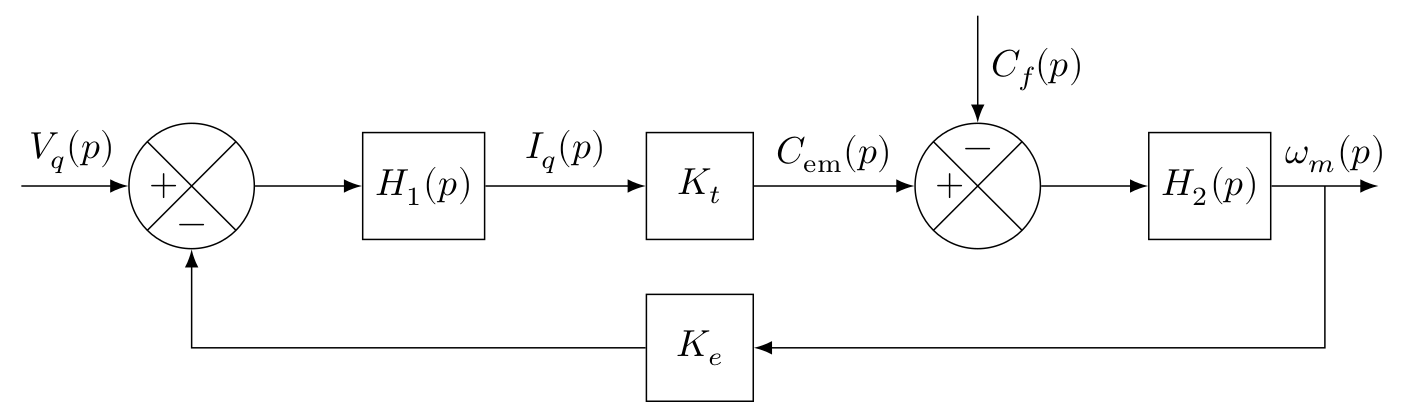
\includegraphics[width=0.7\linewidth]{img/fig14.png}
 \end{center}
  \caption{Schéma bloc de la machine}
\label{fig14}
\end{figure}

\vspace{-0.5cm}

\question{À partir des équations temporelles \ref{eq3} et \ref{eq4}, déterminer les expressions de $H_1(p)$ et $H_2(p)$ du schéma bloc de la figure \ref{fig14}.}

\question{En déduire la fonction de transfert $T(p)=\dfrac{I_q(p)}{V_q(p)}$ sous forme canonique dans le cas où $C_f(p)=0$.}

\begin{table}[!ht]
\begin{center}
 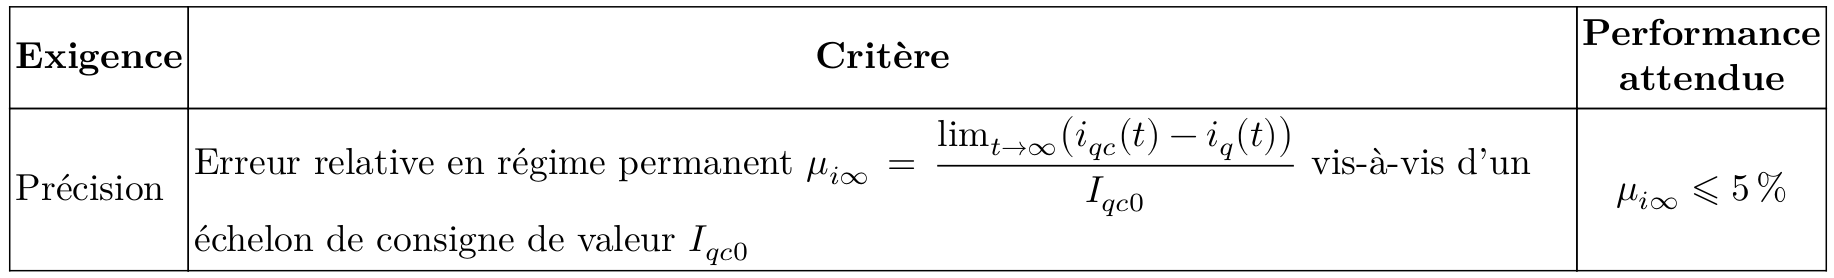
\includegraphics[width=0.85\linewidth]{img/tab05.png}
 \end{center}
  \caption{Détail de l'exigence 5}
\label{tab05}
\end{table}

Pour la suite, et indépendamment des résultats précédents, il est pris
$T(p)=\dfrac{K_0\tau_0p}{(1+\tau_ep)(1+\tau_mp)}$ avec $\tau_e=0.4ms$,
$\tau_m=26ms$ et $K_0\tau_0=0.1s\cdot \Omega^{-1}$.

La boucle d'asservissement de courant est représentée sur la figure \ref{fig15} où $C_1(p)$ représente le correcteur PI de
fonction de transfert $C_1=K_1\dfrac{1+\tau_ip}{\tau_ip}$ avec $\tau_i=\tau_m$.

\begin{figure}[!ht]
\begin{center}
 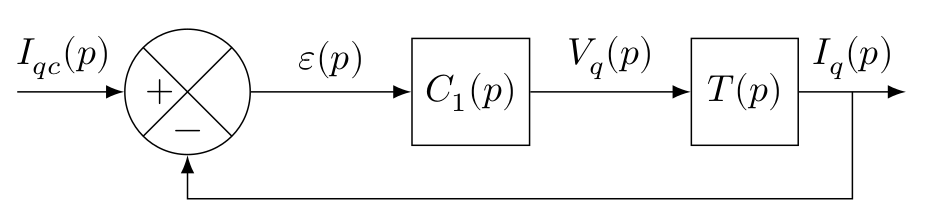
\includegraphics[width=0.5\linewidth]{img/fig15.png}
 \end{center}
  \caption{Schéma bloc de l'asservissement de courant}
\label{fig15}
\end{figure}

\vspace{-0.5cm}

\question{Déterminer l'erreur en régime permanent $\mu_{i\infty}$ pour une consigne en échelon de courant d'amplitude 1 A. Déterminer la valeur de $K_1$ à choisir vis-à-vis des exigences de l'asservissement de courant en terme
de précision données dans le tableau \ref{tab05}.}

~\

La valeur de $K_1$ est supposée assez grande pour considérer par la suite la boucle de courant comme parfaite. L'égalité $I_{qc}(p)=I_{q}(p)$ est donc admise.

La motorisation et sa commande en courant étant maintenant validées, c'est l'étude de l'asservissement en vitesse des motorisations qui va permettre d'analyser le suivi de trajectoire.

\section{Validation du suivi de trajectoire de la base TC200}

Le modèle de connaissance précédent peut désormais être utilisé pour valider par simulation les performances de l'asservissement de vitesse de la base TC200 puis le suivi de trajectoire.

\paragraph{Objectif} Valider l'asservissement de vitesse mis en place pour que la base TC200 se déplace suivant la trajectoire de consigne souhaitée.

\subsection{Étude l'asservissement de vitesse d'un moteur}

\paragraph{Objectif} Vérifier les exigences de la boucle de vitesse en termes de stabilité, précision et rapidité.

\newpage

\begin{table}[!ht]
\begin{center}
 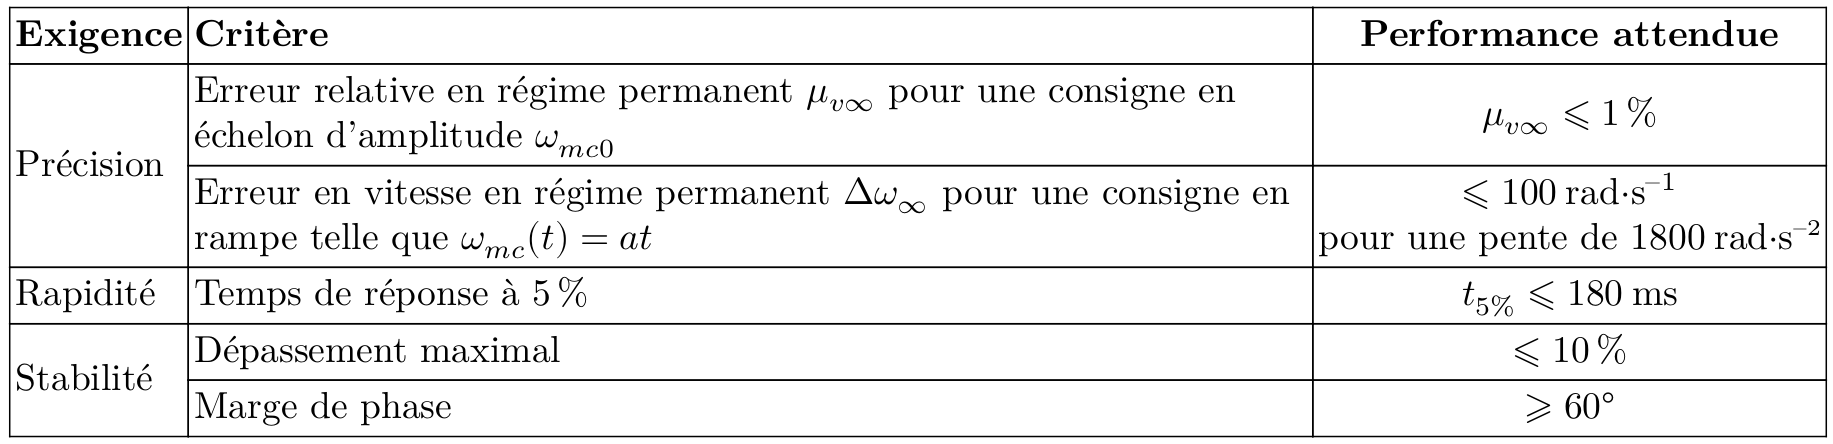
\includegraphics[width=0.95\linewidth]{img/tab08.png}
 \end{center}
  \caption{Exigences de la boucle de vitesse}
\label{tab08}
\end{table}



La boucle de courant étant supposée parfaite, le schéma bloc de la figure \ref{fig19} correspond à l'asservissement de vitesse d'une des motorisations. Le modèle est considéré pour le moment non perturbé, c'est-à-dire $C_f(p)=0$.

\begin{figure}[!ht]
\begin{center}
 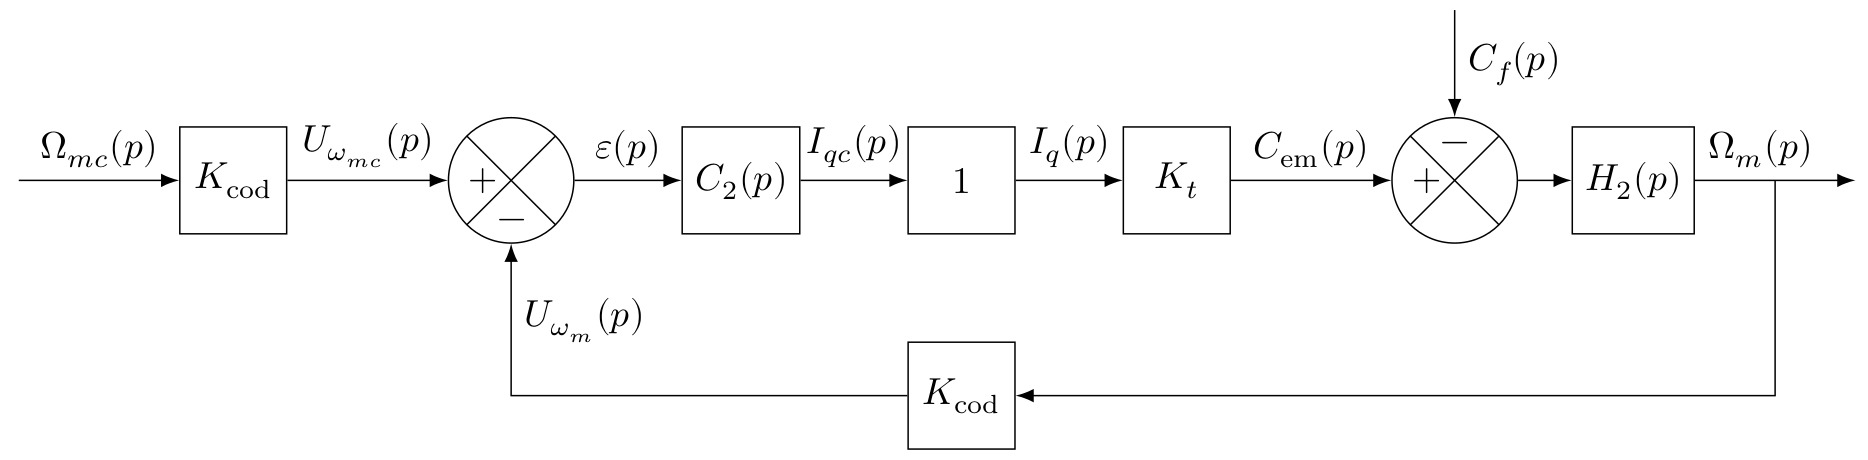
\includegraphics[width=0.95\linewidth]{img/fig19.png}
  \caption{Schéma bloc de l'asservissement de vitesse}
\label{fig19}
 \end{center}
\end{figure}

\vspace{-1cm}

\begin{table}[!ht]
\begin{center}
 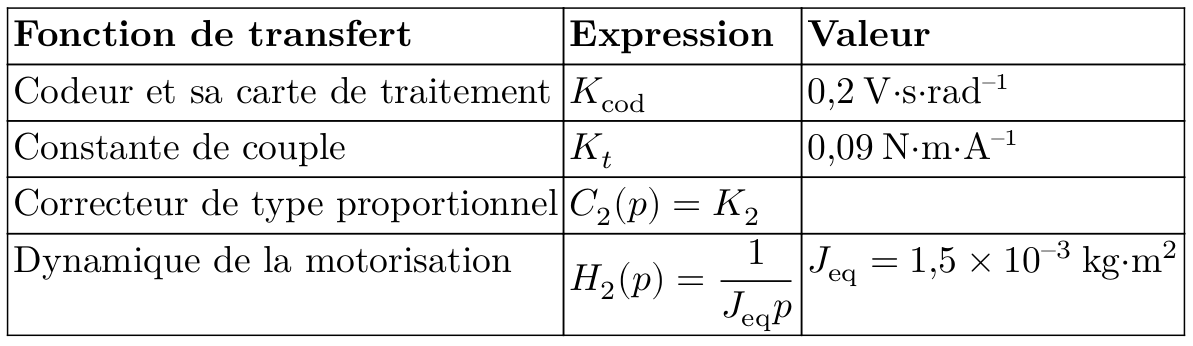
\includegraphics[width=0.7\linewidth]{img/tab09.png}
  \caption{Fonctions de transfert utilisées}
\label{tab09}
 \end{center}
\end{table}

~\

\vspace{-2cm}

\question{Déterminer la fonction de transfert en boucle fermée $K_{BF}(p)=\dfrac{\Omega_m(p)}{\Omega_{mc}(p)}$ pour $C_f(p)=0$.}

\question{Justifier que cet asservissement est stable.}

\question{Déterminer la condition sur $K_2$ afin de satisfaire l'exigence de rapidité du tableau \ref{tab08}.}

\question{Calculer l'erreur relative en régime permanent $\mu_{v\infty}$ pour une consigne de vitesse en échelon de valeur $\omega_{mc0}$.}

~\

Les diagrammes de Bode de la FTBO sont tracés à la figure \ref{fig20}.

\begin{figure}[!ht]
\begin{center}
 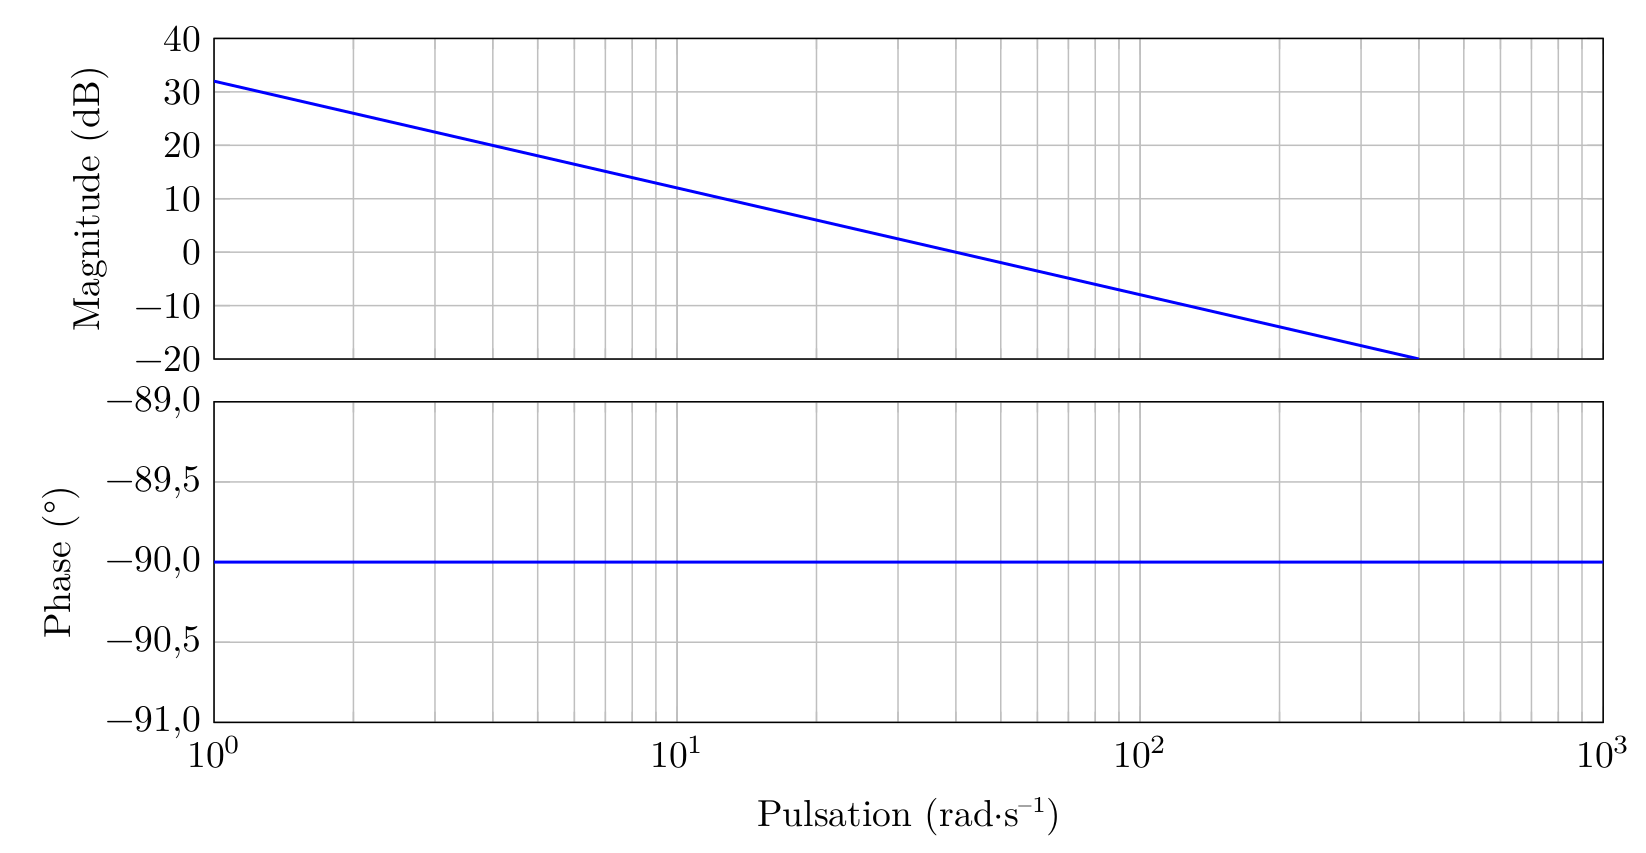
\includegraphics[width=0.85\linewidth]{img/fig20.png}
  \caption{Diagrammes de Bode de la FTBO}
\label{fig20}
 \end{center}
\end{figure}

\newpage

\question{Identifier la valeur de $K_2$ qui a été réellement choisie par le constructeur.}

\question{À partir de cette valeur, calculer l'erreur en vitesse en régime permanent $\Delta_{\omega\infty}$ pour une consigne de vitesse en rampe de pente $a$ et valider le critère de précision des exigences du tableau \ref{tab08}.}

~\

L'asservissement de vitesse non perturbé de la motorisation étant validé, il s'agit maintenant de vérifier la qualité du suivi de trajectoire de la base TC200.

\subsection{Validation des performances du suivi de trajectoire}

\paragraph{Objectif} Analyser et commenter les performances du suivi de trajectoire de la base TC200.

Le modèle complet de simulation des performances du suivi de trajectoire mettant en \oe uvre les quatre motorisations est mis en place. Il reprend l'ensemble des différents modèles de connaissance mis en place dans l'ensemble du sujet.

Les vitesses et la trajectoire de consignes sont représentées sur la figure \ref{fig21}.


\begin{table}[!ht]
\begin{center}
 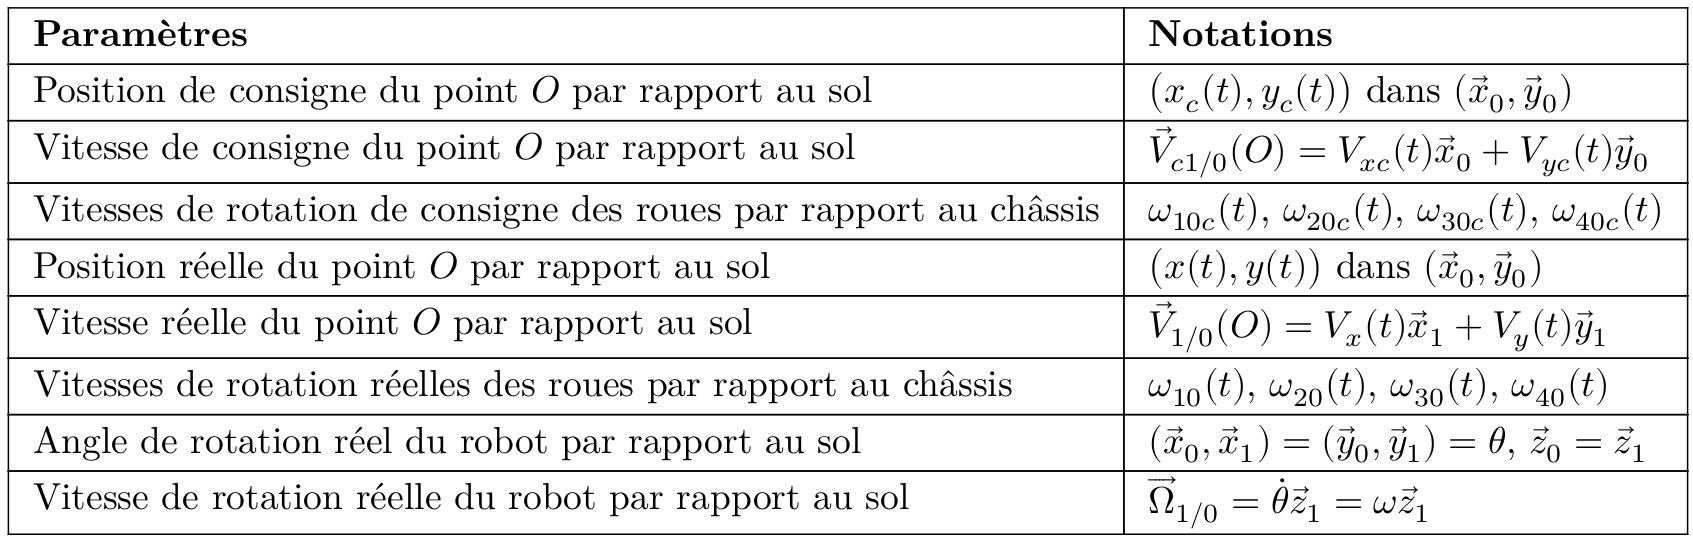
\includegraphics[width=0.75\linewidth]{img/tab06.png}
  \caption{Notations utilisées}
\label{tab06}
 \end{center}
\end{table}

\question{En se référant au tableau \ref{tab06}, proposer l'expression littérale de l'écart entre la trajectoire de consigne et la trajectoire réelle en fonction du temps, en faisant apparaître les paramètres $x_c(t)$, $y_c(t)$, $x(t)$ et $y(t)$.}

~\

Une première simulation est réalisée sans perturbation, c'est-à-dire avec $C_f=0$. La figure \ref{fig22} représente alors l'écart simulé entre la trajectoire réelle et la trajectoire de consigne.

\question{Conclure quant au respect de l'exigence 1.1.1.}

~\

Le suivi de trajectoire non perturbé ayant été étudié, il est nécessaire d'évaluer la contribution du frottement sur la qualité du suivi de trajectoire. Pour cela, la valeur du couple de frottement ramené au niveau de chaque rotor moteur (mais différent pour chaque motorisation) est évalué et introduit dans le modèle de simulation. De plus, un couple résistant aléatoire, différent pour chaque motorisation, est ajouté dans le modèle de simulation pour simuler des perturbations variables à chaque contact roue sol. Différentes courbes issues de cette simulation sont fournies à la figure \ref{fig23}.

~\

\question{Conclure quant au respect de l'exigence 1.1.1 dans ce cas. Proposer une solution technologique permettant de satisfaire l'exigence de précision de positionnement.}

\section{Conclusion}

\question{Conclure vis-à-vis de l'étude menée sur l'utilisation et l'intérêt de la base TC200 dans l'application demandée. Expliquer également pourquoi une précision de positionnement de 1 cm de la base TC200 est suffisante
pour le vissage de vis d'un diamètre variable de 0,4 à 2 cm.}

\question{D'après les données disponibles, notamment la figure \ref{fig24}, présenter les étapes de la fabrication du châssis du robot, de la mise en forme du brut à la finition.}

\question{Décrire 3 différentes solutions techniques pour cette mise en forme du brut (qui permet d'obtenir la géométrie de la pièce de la figure \ref{fig24}) et l'utilisation de celle qui vous parait la plus probable.}

\begin{figure}[!ht]
\begin{center}
 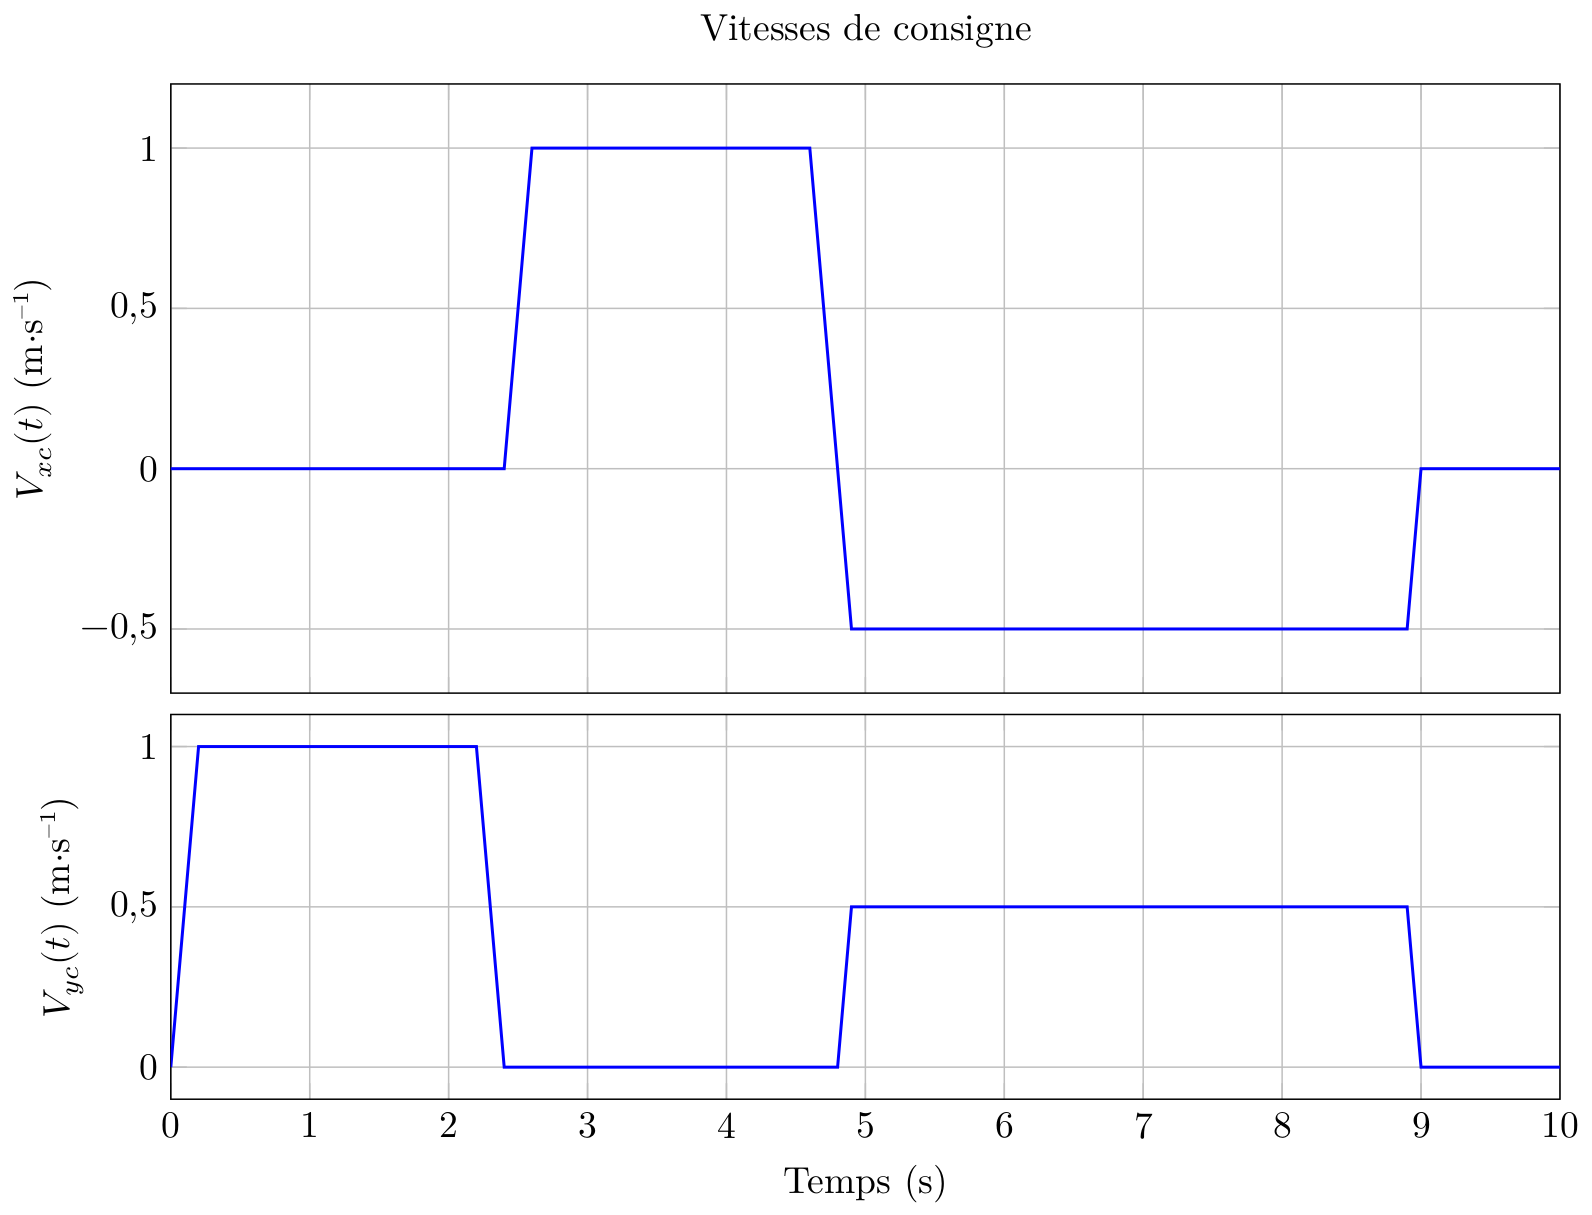
\includegraphics[width=0.8\linewidth]{img/fig21_1.png} \\
 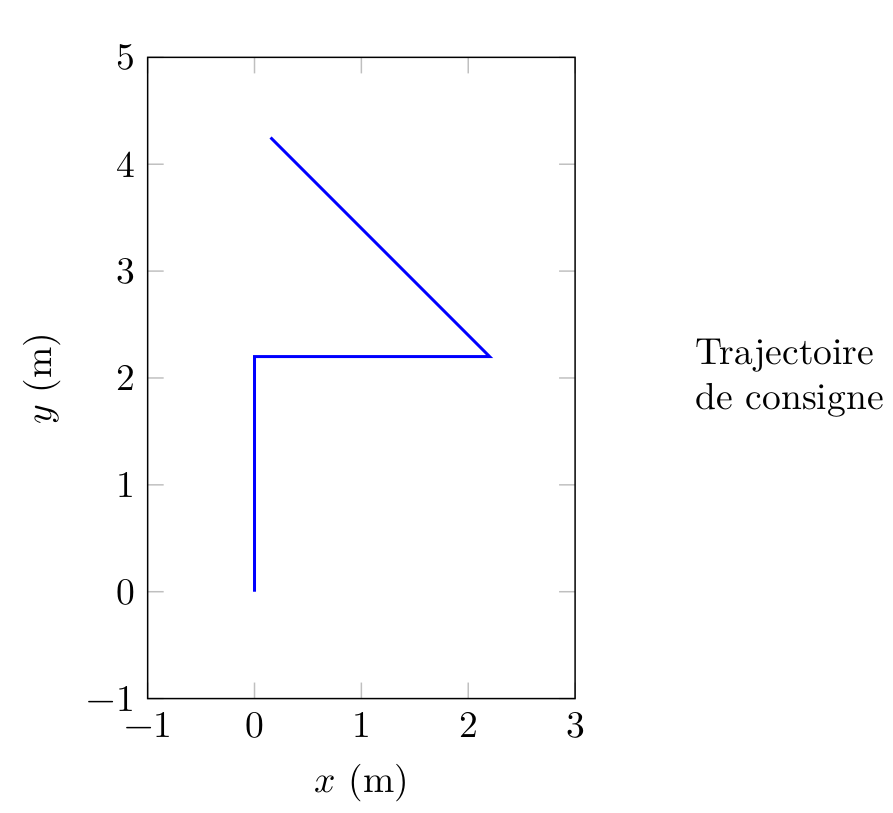
\includegraphics[width=0.4\linewidth]{img/fig21_2.png}
 \end{center}
  \caption{Vitesses de consigne en fonction du temps et trajectoire de consigne}
\label{fig21}
\end{figure}

\begin{figure}[!ht]
\begin{center}
 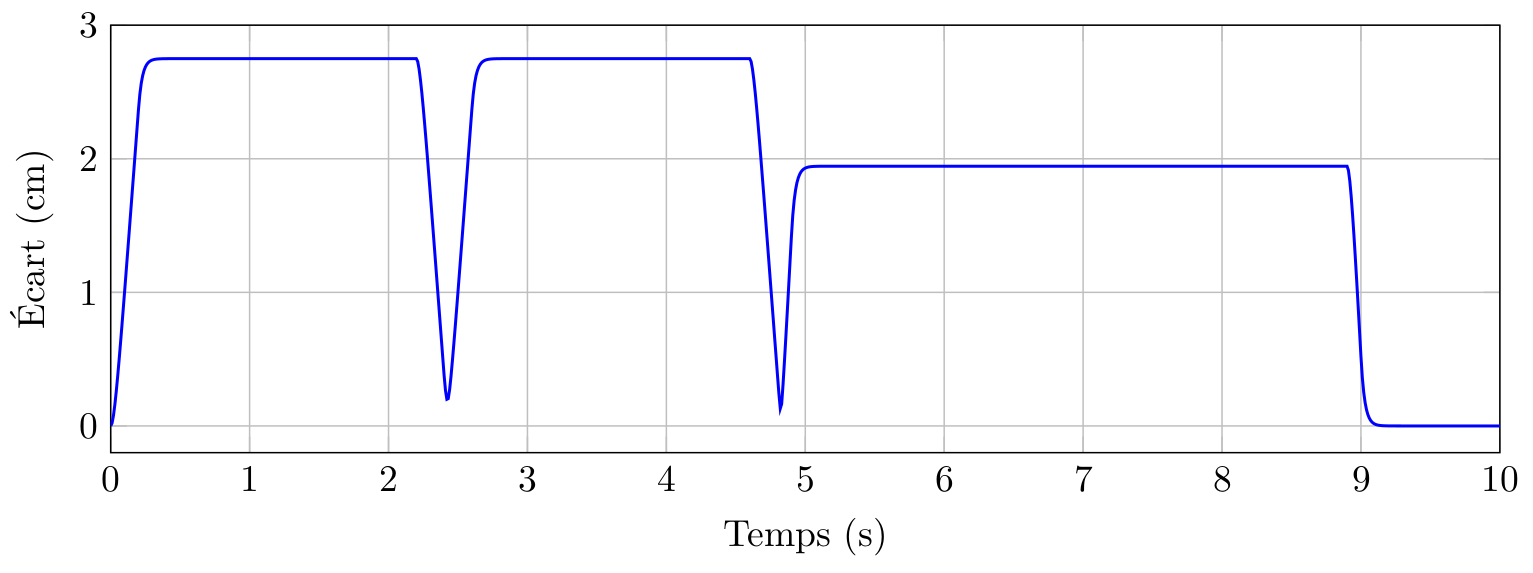
\includegraphics[width=0.8\linewidth]{img/fig22.png}
 \end{center}
  \caption{Écart entre la trajectoire de consigne et la trajectoire réelle lorsque $C_f=0$}
\label{fig22}
\end{figure}

\begin{figure}[!ht]
\begin{center}
 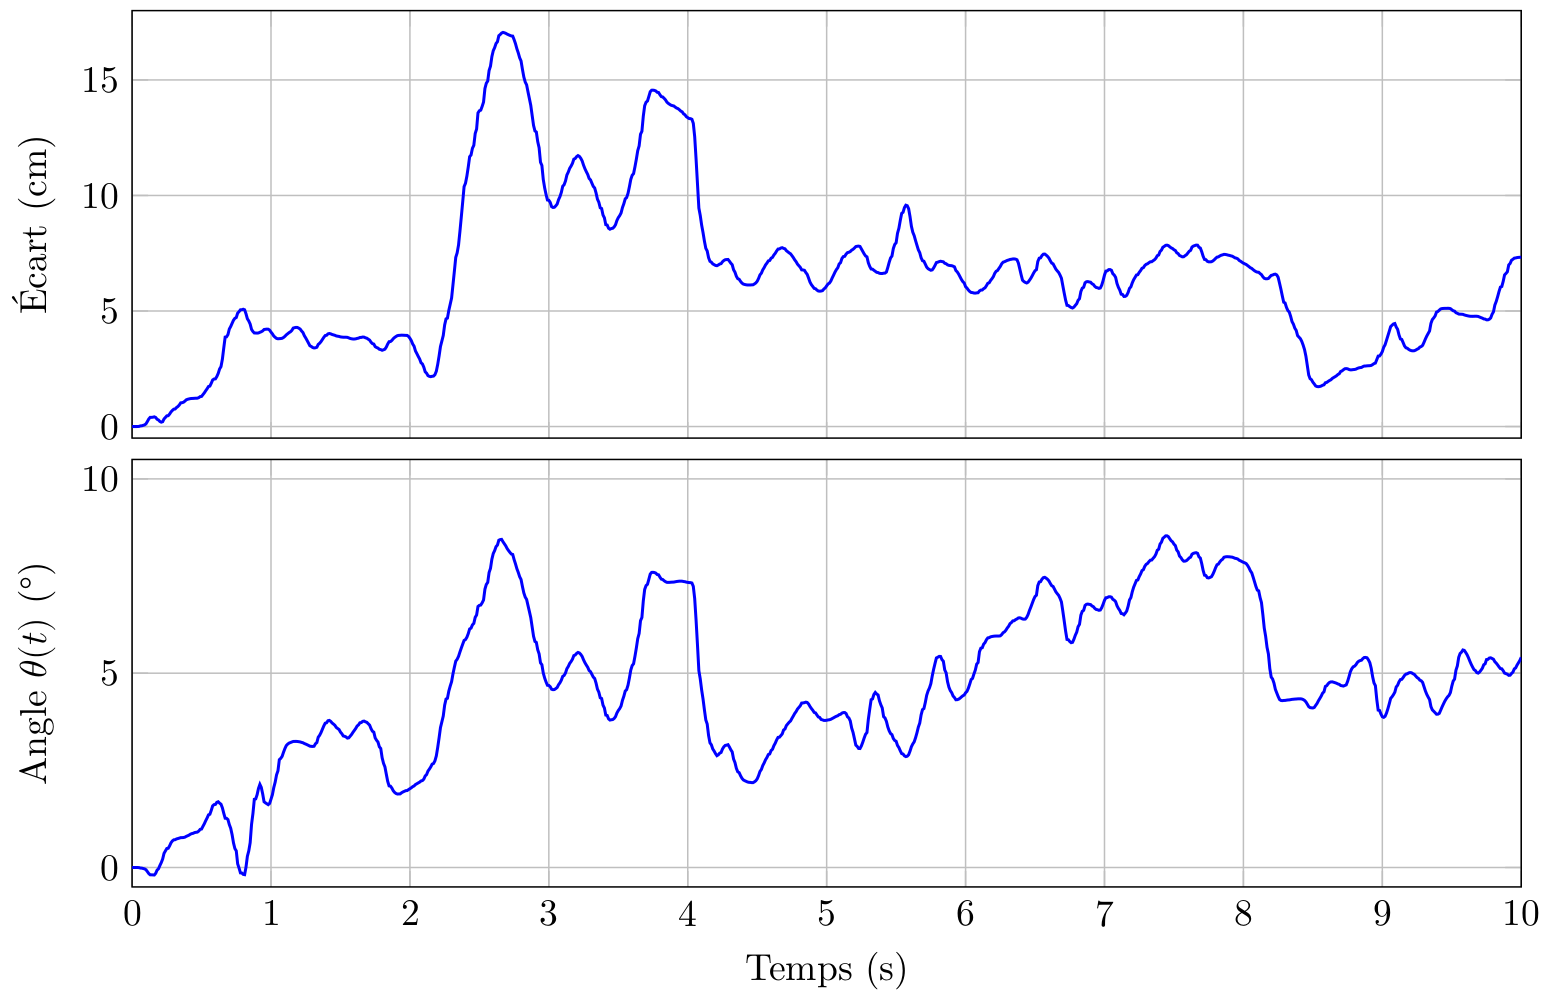
\includegraphics[width=0.8\linewidth]{img/fig23_1.png} \\
 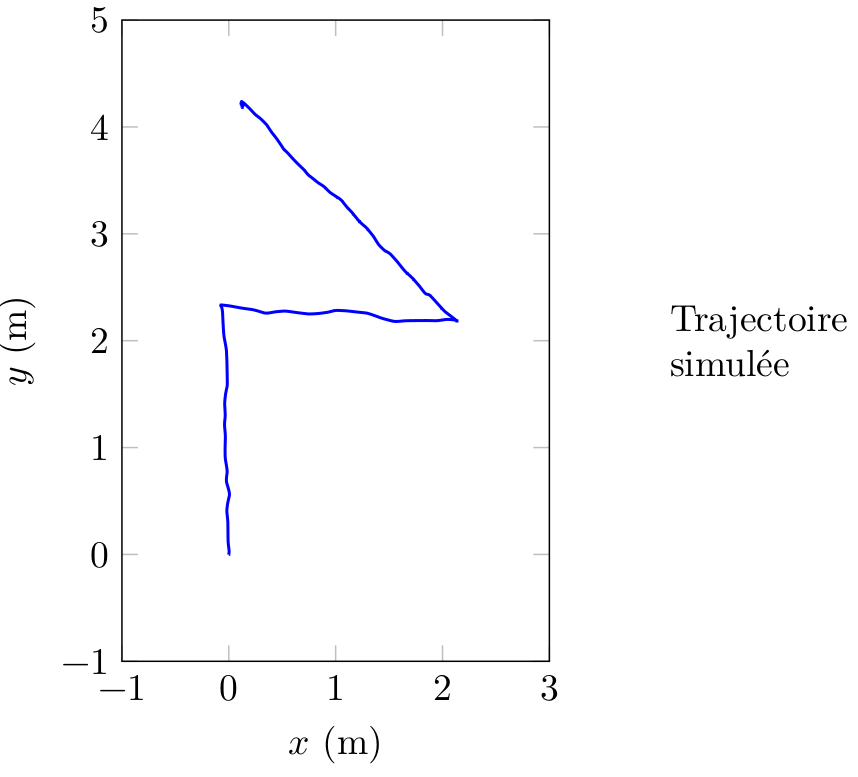
\includegraphics[width=0.4\linewidth]{img/fig23_2.png}
 \end{center}
  \caption{Simulation avec des couples de perturbation aléatoires sur chaque moteur}
\label{fig23}
\end{figure}

\begin{figure}[!ht]
\begin{center}
 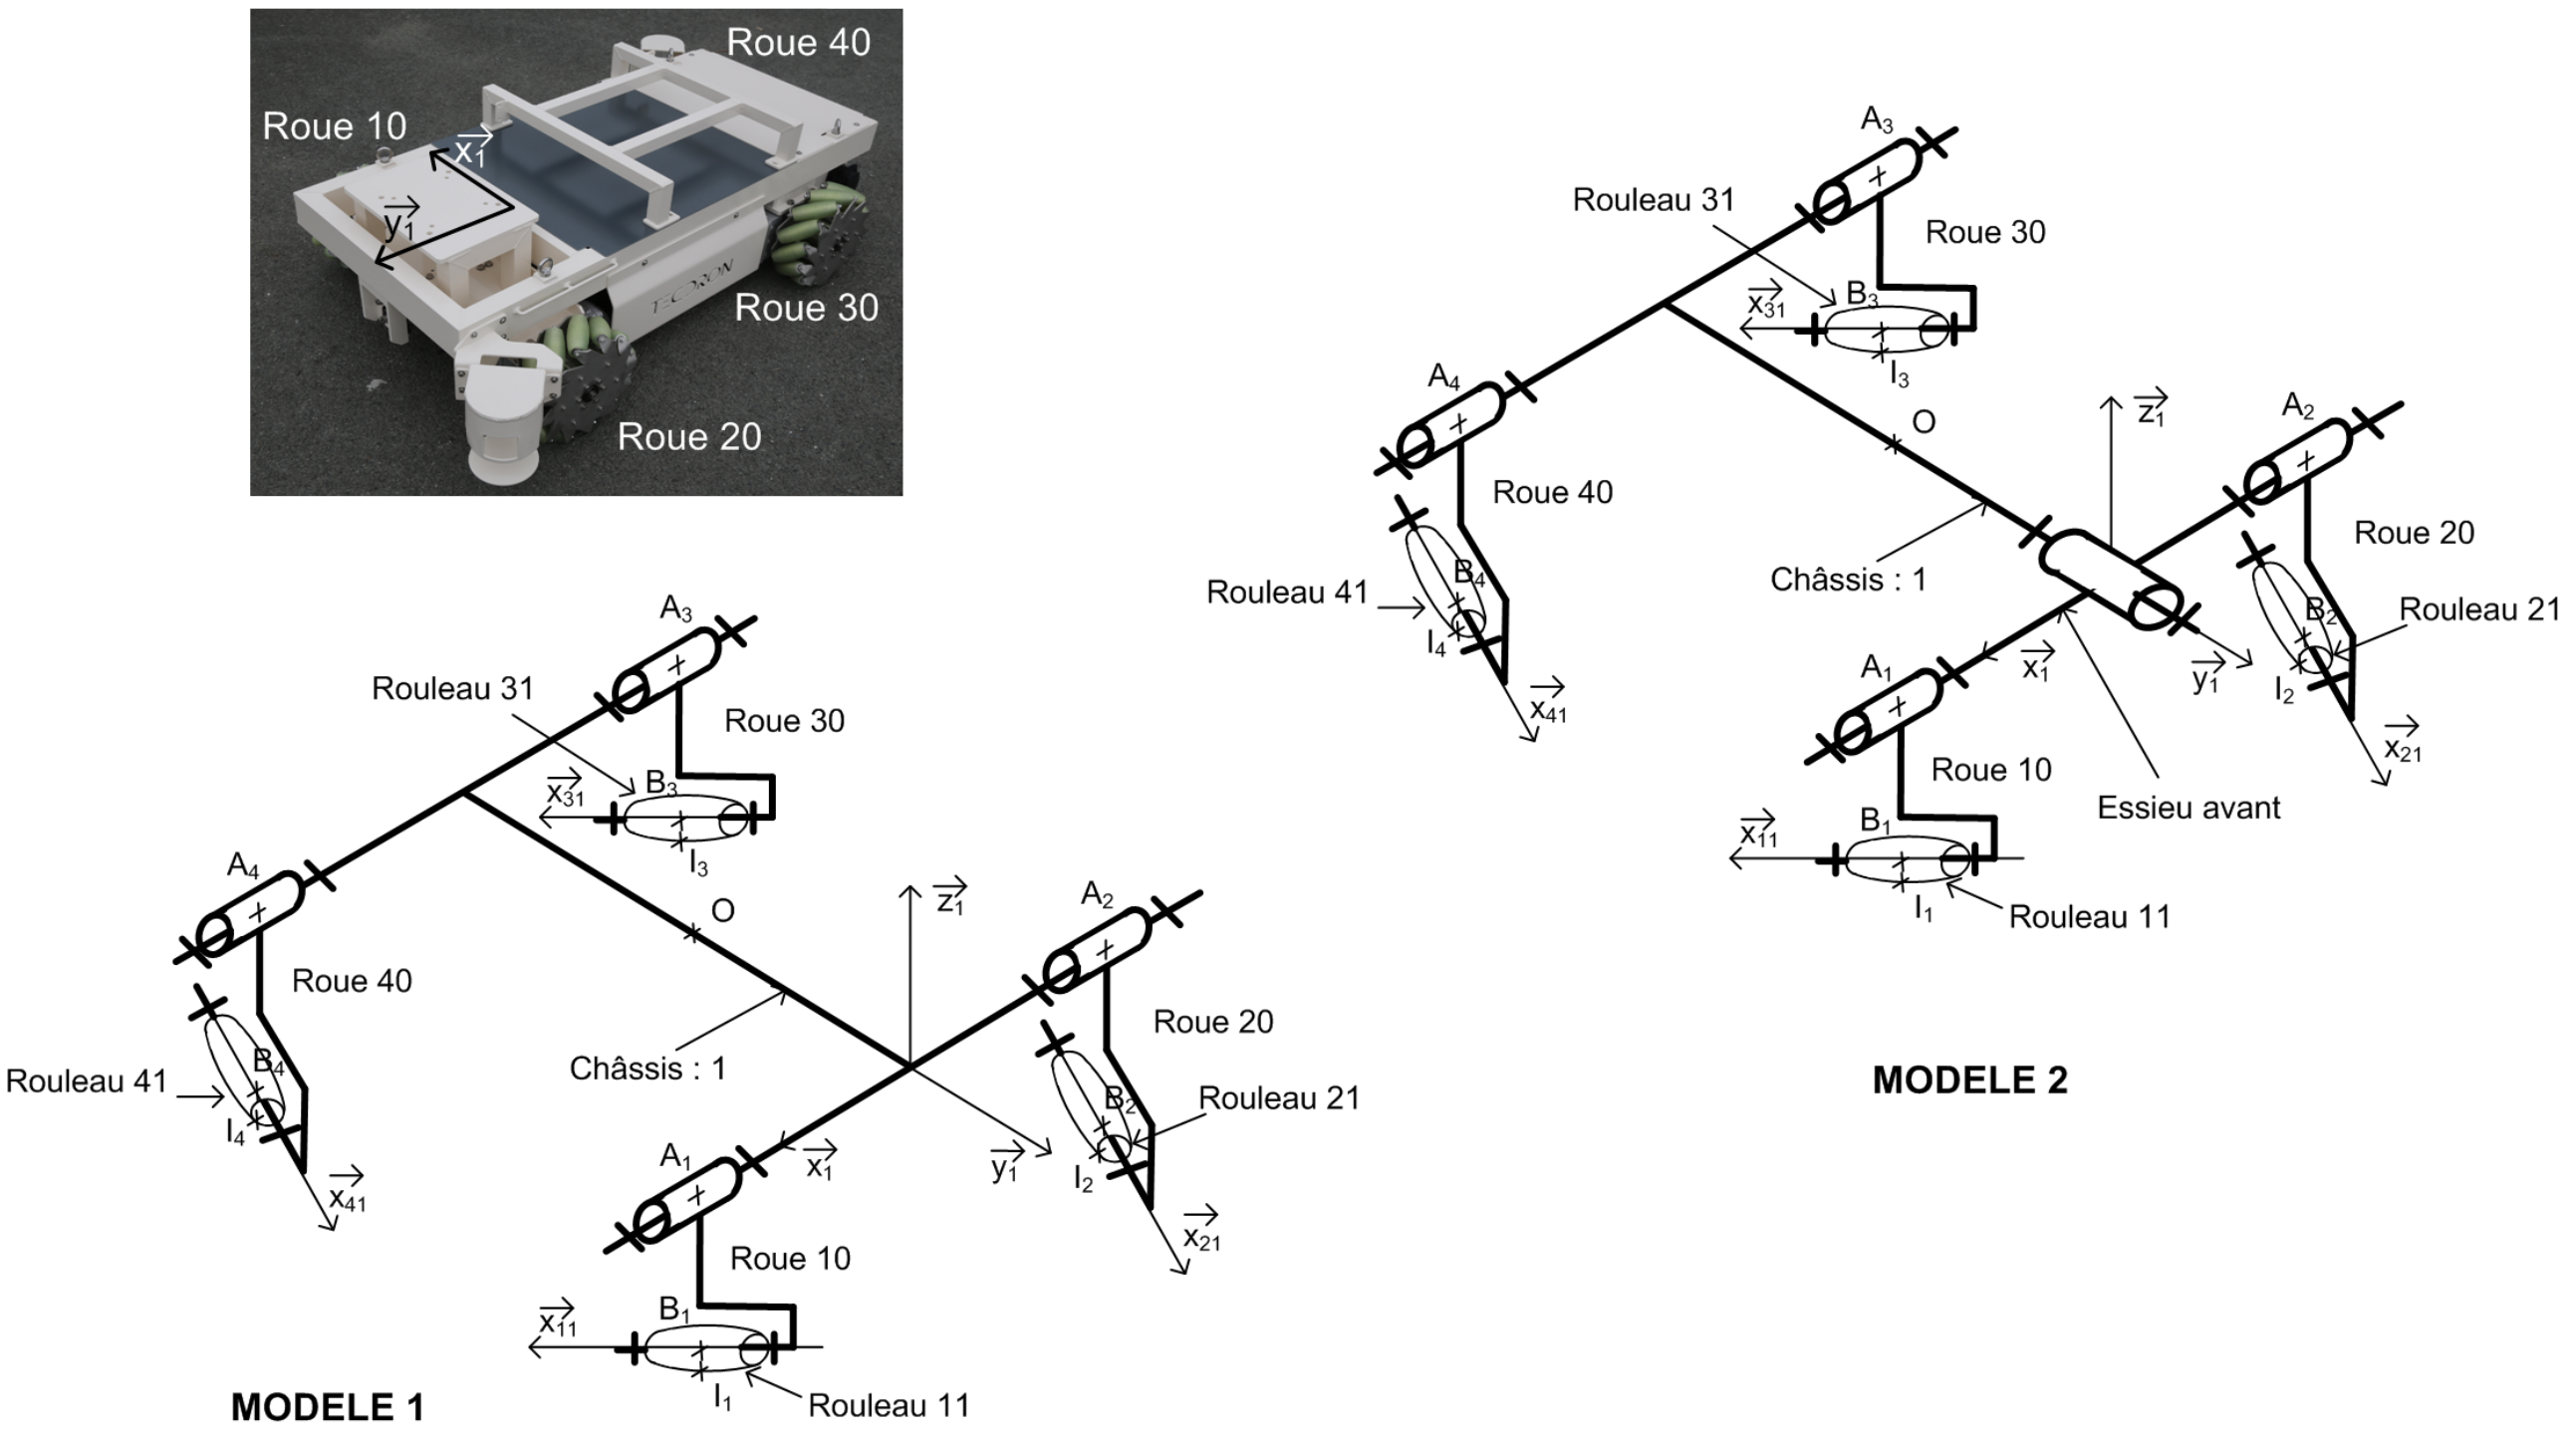
\includegraphics[angle=90,width=0.75\linewidth]{img/fig24.png}
 \end{center}
  \caption{Deux modèles cinématiques de la base TC200}
\label{fig24}
\end{figure}

\begin{figure}[!ht]
\begin{center}
 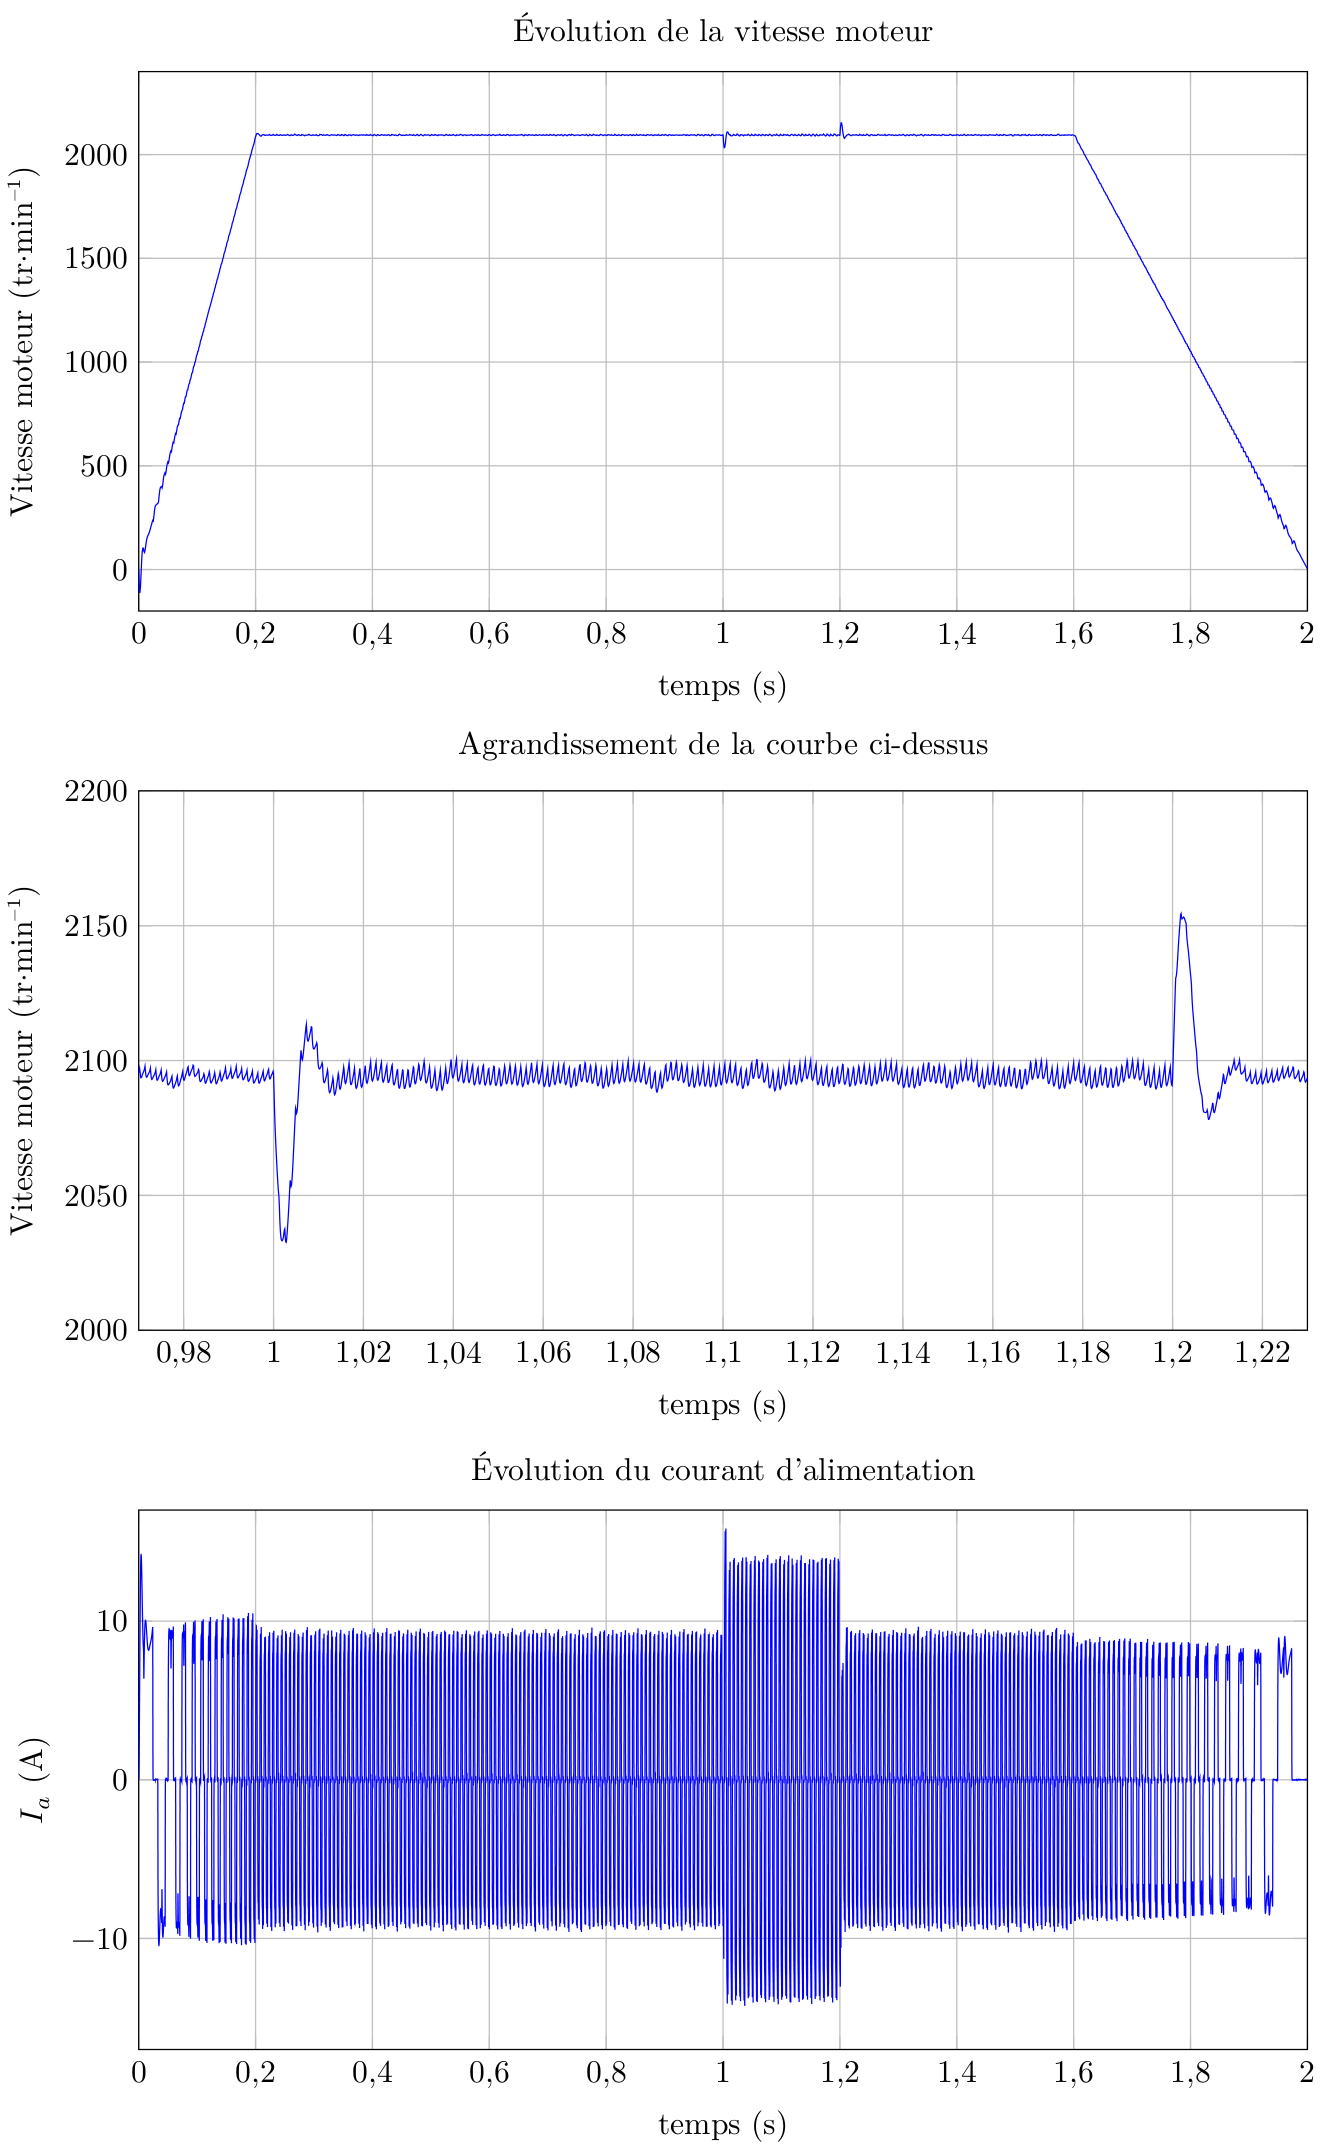
\includegraphics[width=0.8\linewidth]{img/fig25.png}
 \end{center}
  \caption{Courbes obtenues avec le modèle multiphysique}
\label{fig25}
\end{figure}

\cleardoublepage

\ifdef{\public}{\pagestyle{documentreponse}}{\pagestyle{correction}}

\reponse{0}{\begin{center}
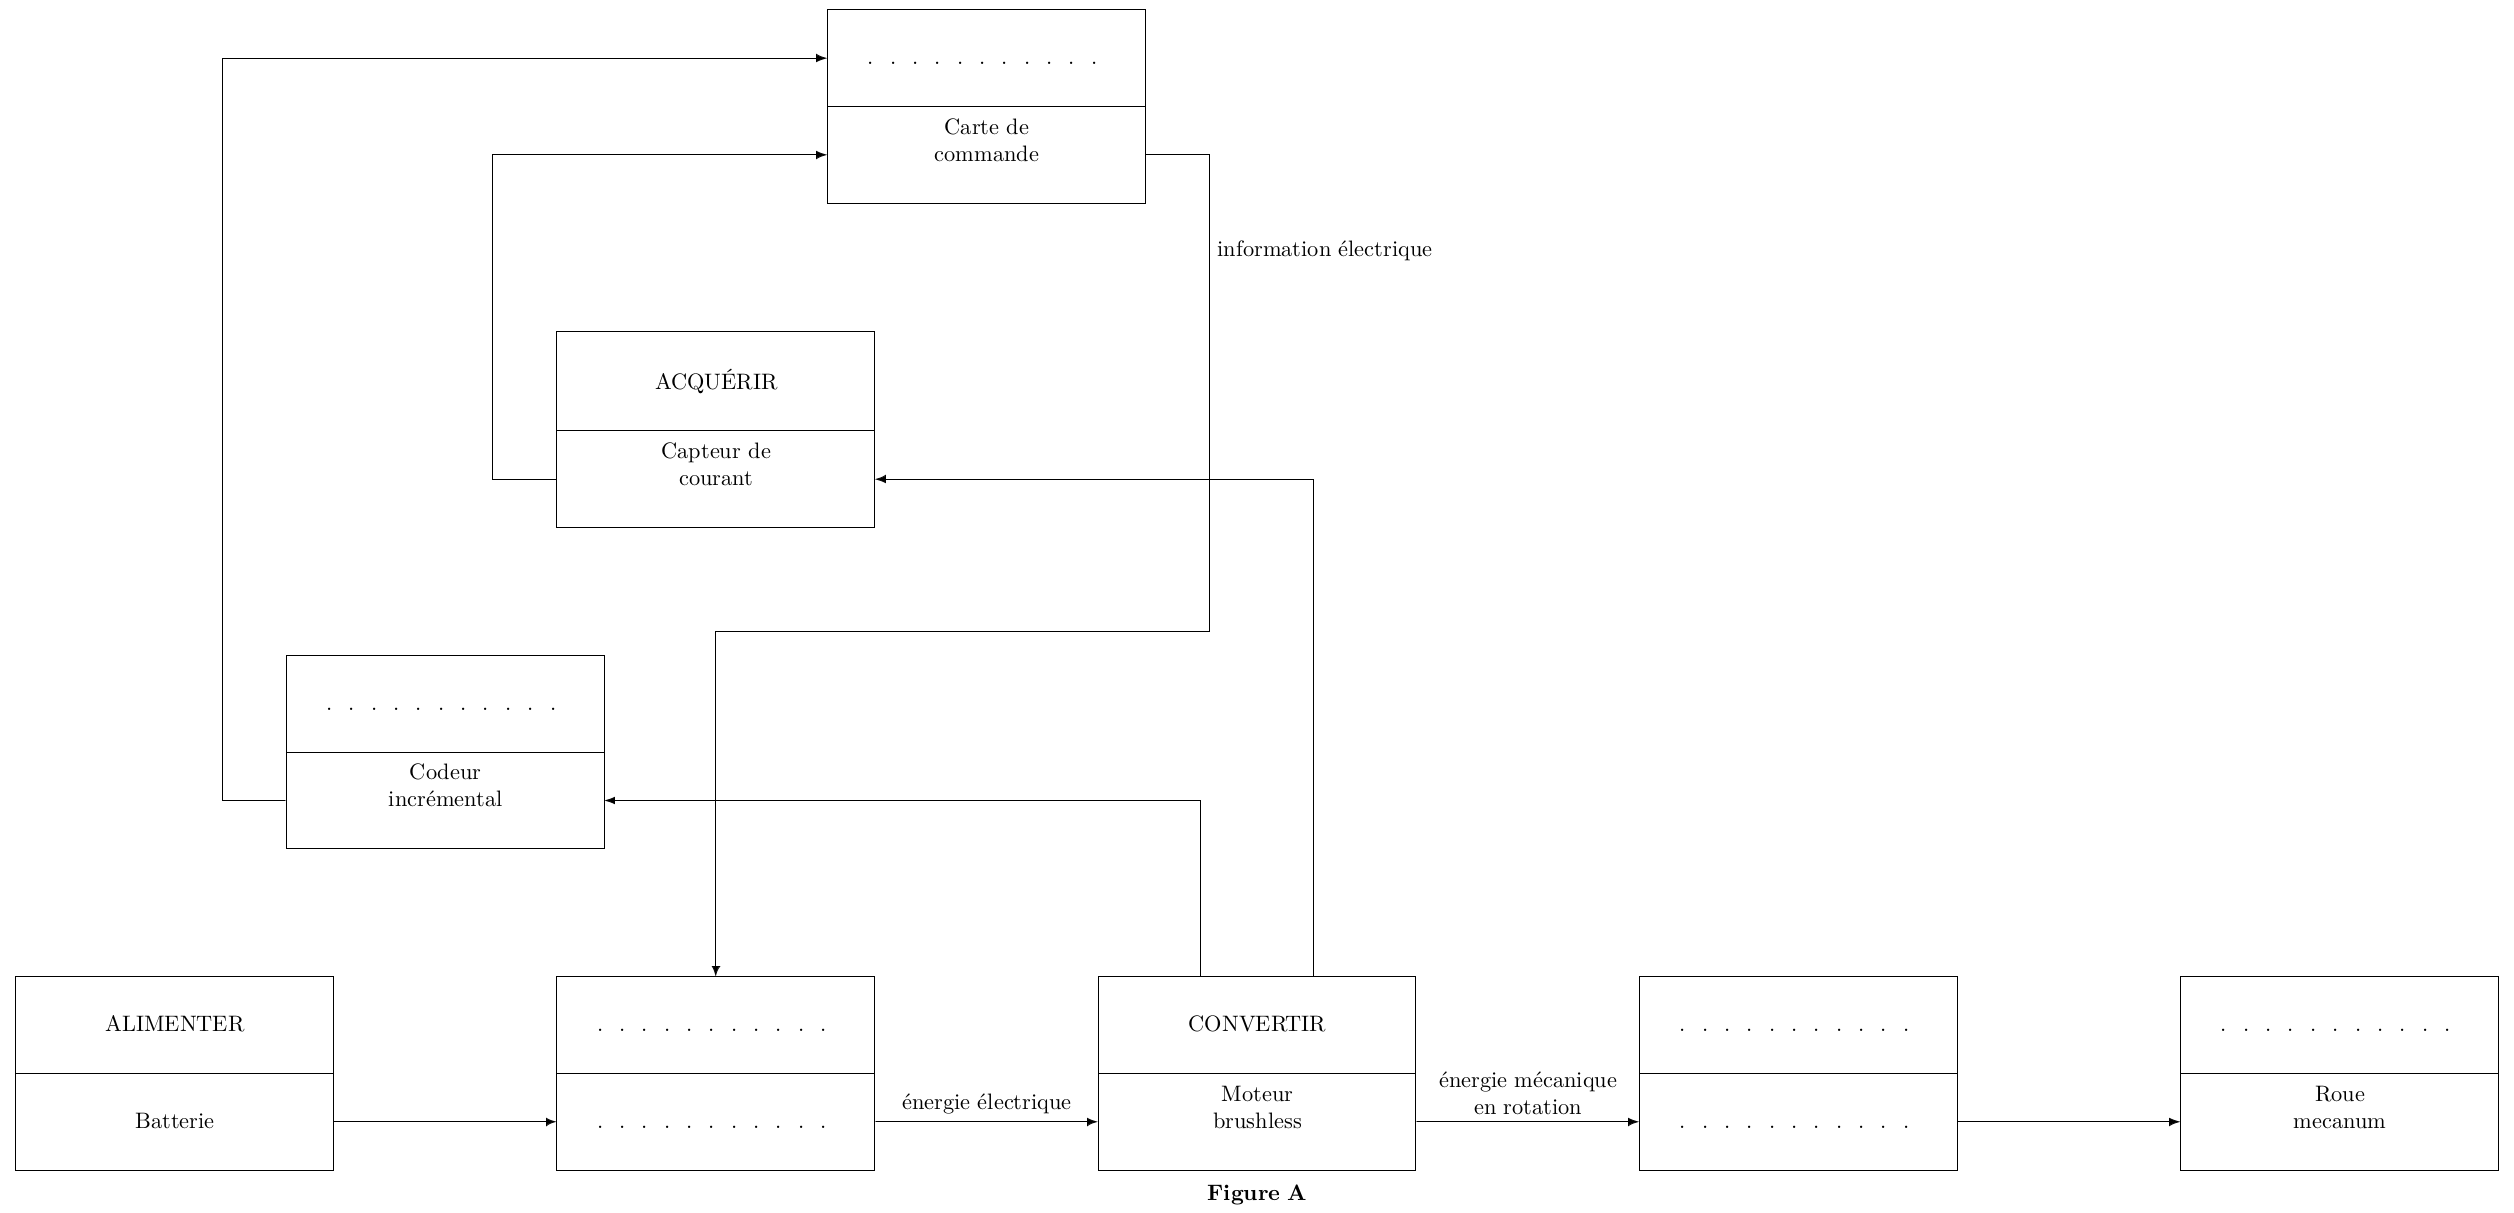
\includegraphics[width=\linewidth]{img/DR01}
\end{center}}{\begin{center}
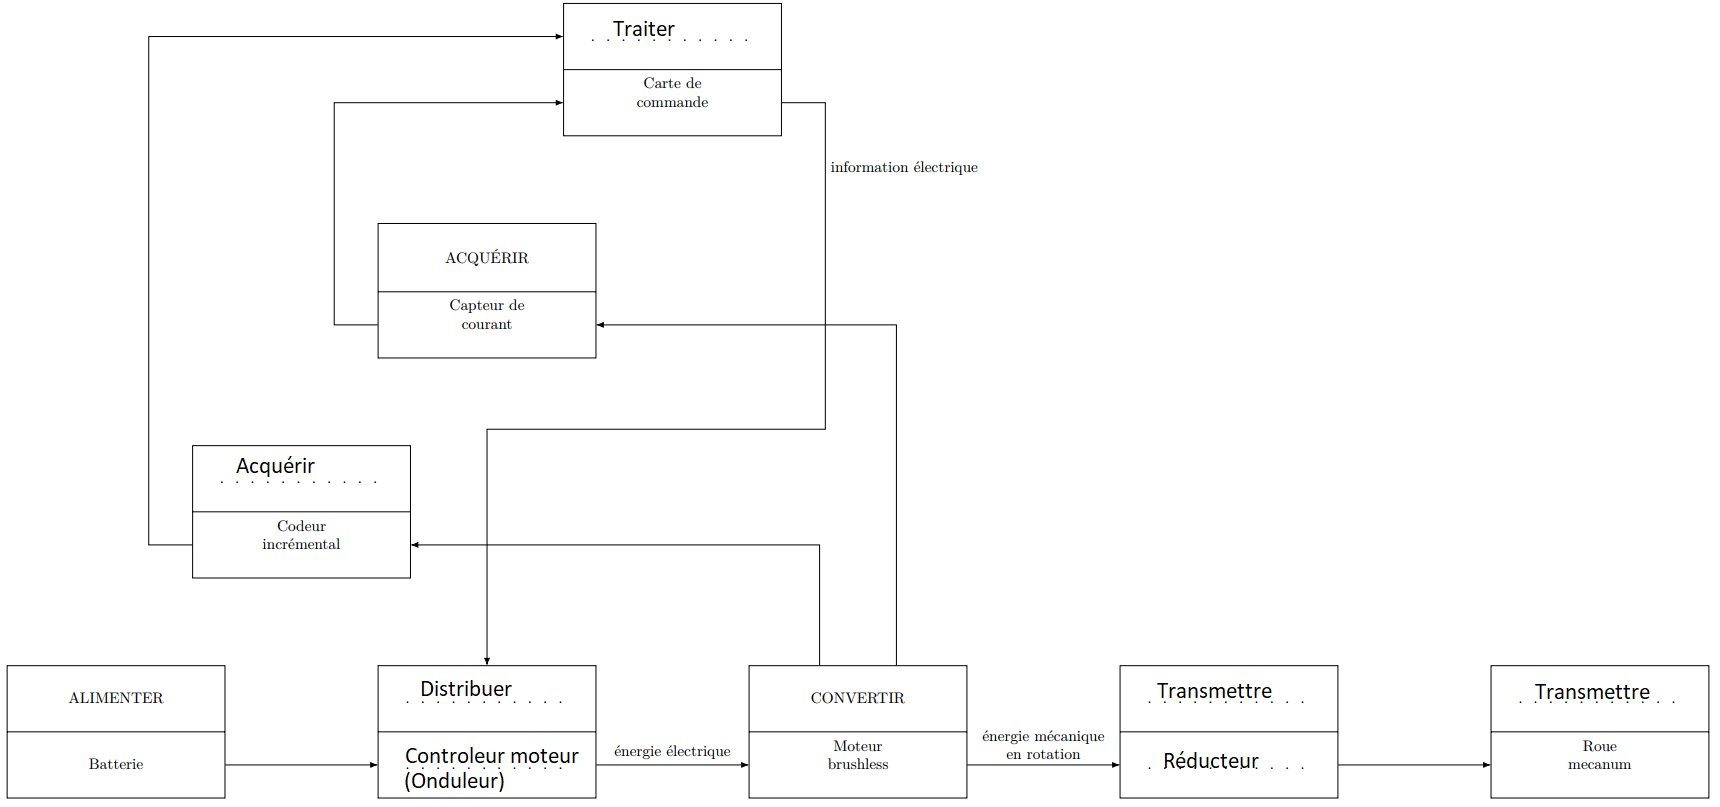
\includegraphics[width=\linewidth]{img/DR01_cor}
\end{center}}


\reponse{2}{
\begin{center}
\begin{tabular}{|>{\centering\arraybackslash}p{6cm}|>{\centering\arraybackslash}p{6cm}|}
\hline
Modèle 1 & Modèle 2 \\
\hline
  &  \\
  &  \\
  &  \\
  &  \\
  &  \\
  &  \\
  &  \\
  &  \\
  &  \\
  &  \\
  &  \\
 \hline
\end{tabular}
\end{center}
}{
\begin{center}
\begin{tabular}{|c|c|}
\hline
Modèle 1 & Modèle 2 \\
\hline
8 pivots et 4 ponctuelles & 9 pivots et 4 ponctuelles \\
$Ns = 8*5 + 4 = 44$ & $Ns = 9*5 + 4 = 49$ \\
\hline
10 pièces & 11 pièces \\
\hline
$h= 44 - 6*(10 - 1)+ 3 + 8 =1$ & $h= 49 - 6*(11 - 1)+ 3 + 8 =0$ \\
\hline
h=1 (hyperstatique) & h=0 (isostatique)\\
\hline
\end{tabular}
\end{center}

Seul le modèle 2 répond au cahier des charges et c'est bien celui retenu par le constructeur.}

\ifdef{\public}{\newpage}

\reponse{6}{}{

$\overrightarrow{V_{I1,11/10}}+\overrightarrow{V_{I1,10/1}}+\overrightarrow{V_{I1,1/0}}=\overrightarrow{0}$

$r\dot{\beta}_{11}\vec{y}_{11}+(r+R)\omega_{10}\vec{y}_1+V_x\vec{x}_1+V_y\vec{y}_1+a\omega\vec{y}_1-b\omega\vec{y}_1=\overrightarrow{0}$


Or, $\vec{y}_{11}=-sin\alpha_{11}\vec{x}_1+cos\alpha_{11}\vec{y}_1=\dfrac{\sqrt{2}}{2}(\vec{x}_1+\vec{y}_1)$

D'où $r\dot{\beta}_{11}\dfrac{\sqrt{2}}{2}(\vec{x}_1+\vec{y}_1)+(r+R)\omega_{10}\vec{y}_1+V_x\vec{x}_1+V_y\vec{y}_1+a\omega\vec{y}_1-b\omega\vec{x}_1=\vec{0}$

Soit, en projetant sur $\vec{x}_1$ et $\vec{y}_1$:

$V_x-b\omega+r\dot{\beta}_{11}\dfrac{\sqrt{2}}{2}=0$

$V_y+a\omega+(r+R)\omega_{10}+r\dot{\beta}_{11}\dfrac{\sqrt{2}}{2}=0$

}

\reponse{6}{}{D'après les équations précédentes, et en substituant $r\dot{\beta}_{11}\dfrac{\sqrt{2}}{2}$, on obtient

$V_y+a\omega+(r+R)\omega_{10}-V_x+b\omega=0$

$\omega_{10}=\dfrac{1}{r+R}\left(-(a+b)\omega+V_x-V_y\right)$

En faisant la même chose pour les équations suivantes, on obtient:

$M=\dfrac{1}{r+R}\left(\begin{array}{c c c}
-(a+b) & 1 & -1 \\
a+b & -1 & -1 \\
a+b & 1 & -1 \\
-(a+b) & -1 & -1 \\
\end{array}\right)$

}

\reponse{6}{}{En faisant le calcul, on trouve

$W_1=\dfrac{1}{r+R}\left(\begin{array}{c}
-1 \\
-1 \\
-1 \\
-1 \\
\end{array}\right)$
$W_2=\dfrac{1}{r+R}\left(\begin{array}{c}
1 \\
-1 \\
1 \\
-1 \\
\end{array}\right)$
$W_3=\dfrac{1}{r+R}\left(\begin{array}{c}
0 \\
-2 \\
0 \\
-2 \\
\end{array}\right)$

On peut retrouver les composantes de $V$ à partir de $W$, il y a 4 équations pour 3 inconnues mais la dernière est une combinaison linéaire des trois autres, donc elle n'est pas nécessaire pour le calcul.

Cette réversibilité est possible car le système est isostatique.
}

\reponse{4}{\begin{center}

~\

\vspace{-1cm}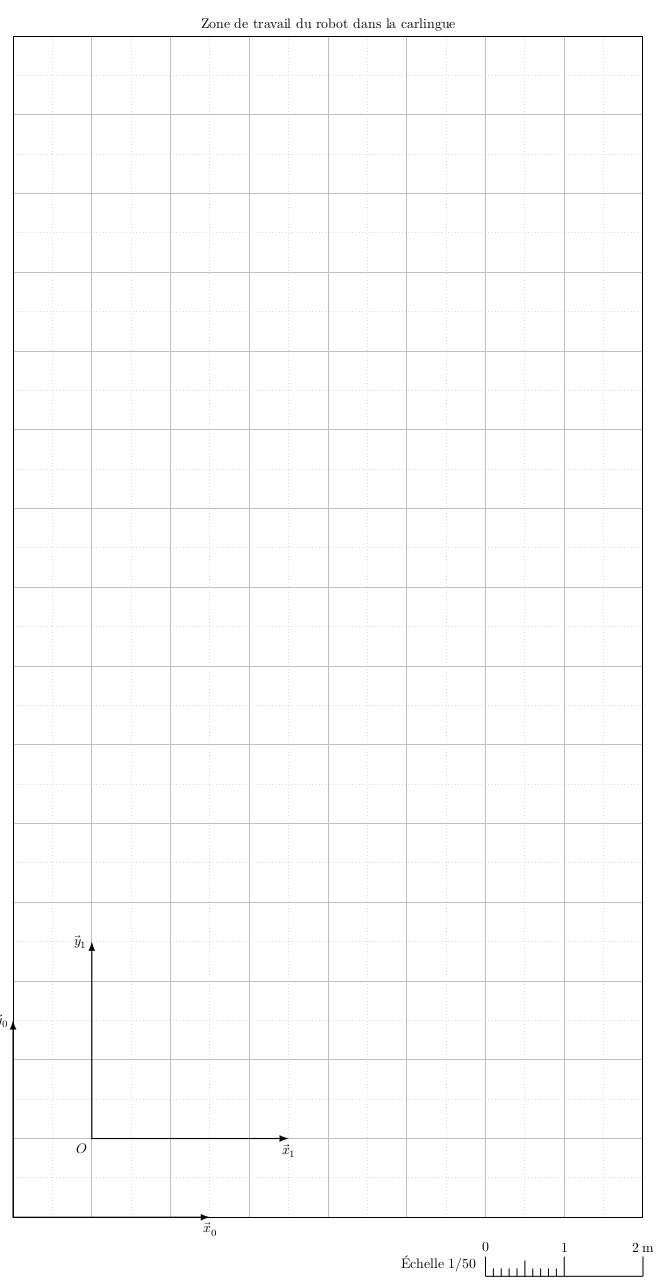
\includegraphics[angle=90,width=\linewidth]{img/DR02}\vspace{-0.5cm}
\end{center}}{

~\

\begin{minipage}{0.5\linewidth}
On peut déterminer:
\begin{itemize}
 \item $V_x(t)=-\dfrac{r+R}{2}\left(\omega_{10}(t)+\omega_{20}(t)\right)$
 \item $V_y(t)=-\dfrac{r+R}{2}\left(\omega_{10}(t)-\omega_{20}(t)\right)$\end{itemize}
  
Avec $\dfrac{r+R}{2}=73mm$.
\end{minipage}\hfill
\begin{minipage}{0.45\linewidth}
\begin{tabular}{|c|c|c|c|}
\hline
 & Durée & $V_x(t)$ & $V_y(t)$ \\
\hline
État 1  & 2s & $0m\cdot s^{-1}$& $1m\cdot s^{-1}$\\
\hline
État 2  & 2s & $1m\cdot s^{-1}$& $0m\cdot s^{-1}$\\
\hline
État 3  & 2s & $-1m\cdot s^{-1}$& $0m\cdot s^{-1}$\\
\hline
État 4  & 2s & $1m\cdot s^{-1}$& $1m\cdot s^{-1}$\\
\hline
État 5  & 2s & $-1m\cdot s^{-1}$& $1m\cdot s^{-1}$\\
\hline
\end{tabular}

\end{minipage}

\begin{center}
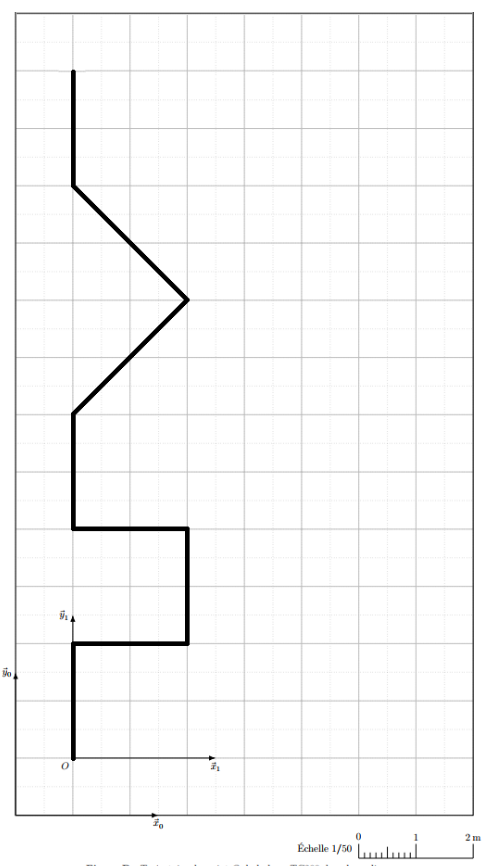
\includegraphics[angle=90,width=\linewidth]{img/DR02_cor}
\end{center}
}

\reponse{7}{}{On prendra les hypothèses d'un problème plan.

En A, liaison pivot : $\left\{T_{0\rightarrow p}\right\}=\left\{\begin{array}{cc}
X_A & ~ \\
Y_A & ~ \\
0 & 0
\end{array}\right\}_A$

En D, liaison ponctuelle : $\left\{T_{0\rightarrow p}\right\}=\left\{\begin{array}{cc}
0 & ~ \\
Y_A & ~ \\
0 & 0
\end{array}\right\}_A$

En B, action F: $\left\{T_{0\rightarrow p}\right\}=\left\{\begin{array}{cc}
0 & ~ \\
F & ~ \\
0 & 0
\end{array}\right\}_B$

En C, action F: $\left\{T_{0\rightarrow p}\right\}=\left\{\begin{array}{cc}
0 & ~ \\
F & ~ \\
0 & 0
\end{array}\right\}_C$

On obtient après avoir tout déplacé en A:
$\left\{\begin{array}{l}
X_A=0\\
2F+Y_A+Y_D=0\\
(2L_1+L_2)Y_D+(2L1+L2)F=0
\end{array}
\right.$
$\left\{\begin{array}{l}
X_A=0\\
Y_A=-F\\
Y_D=-F
\end{array}
\right.$}

\reponse{4}{}{$Re=450MPa$, $Rm=60MPa$, $A\%=2,45$.}

\reponse{4}{}{$\sigma_{max}=\dfrac{F\cdot L_1\cdot 64\cdot d}{\pi\cdot d^4\cdot 2}=\dfrac{500\cdot 50\cdot 64\cdot 15}{\pi\cdot 15^4\cdot 2}=75MPa$}

\reponse{4}{}{$\sigma_{max}\leq \dfrac{Re}{5}$, donc l'exigence est respectée.}

\reponse{4}{}{Un onduleur est un dispositif d'électronique de puissance permettant de générer des tensions et des courants alternatifs à partir d'une source d'énergie électrique continue.}

\newpage

\reponse{6}{}{Grâce aux équations du moteur, on trouve:

$H_1(p)=\dfrac{1}{R_{eq}+L_{eq}p}$ et $H_2(p)=\dfrac{1}{J_{eq}p}$}

\reponse{6}{}{La fonction de transfert est $T(p)=\dfrac{\dfrac{J_{eq}}{KeK_t}p}{1+\dfrac{J_{eq}R_{eq}}{K_eK_t}p+\dfrac{J_{eq}L_{eq}}{K_eK_t}p^2}$}

\reponse{6}{}{On commence par calculer $\epsilon(p)=\dfrac{\tau_i(1+\tau_ep)}{\tau_i+K_1K_0\tau_0+\tau_i\tau_ep}I_{qc}(p)$

Donc, $\mu_{i\infty}=\lim\limits_{p\rightarrow 0}p\epsilon(p)=\dfrac{\tau_i}{\tau_i+K_1K_0\tau_0}$

Il faut que cette erreur soit inférieure à 5\% d'après le tableau\ref{tab05}.

Donc, $K_1\geq\dfrac{\tau_i(1-0,05)}{0,05K_0\tau_0}$ $K_1\geq\dfrac{0,026 \cdot 0,95}{0,05\cdot 0,1}$ donc $K_1\geq 5$
}

\reponse{7}{}{$H_{BF}=\dfrac{1}{1+\dfrac{J_{eq}}{K_2K_tK_{cod}}p}$}

\reponse{2}{}{Il s'agit d'une fonction du premier ordre, il est donc toujours stable.}

\reponse{6}{}{Le temps de réponse est $3\tau$, donc $3\dfrac{J_{eq}}{K_2K_tK_{cod}}\leq180ms$, donc $K_2\geq\dfrac{5\cdot 10^{-4}}{2\cdot 9\cdot 2\cdot 10^{-5}}$, donc $K_2\geq1,4$}

\ifdef{\public}{\newpage}

\reponse{5}{}{Comme il y a un intégrateur, l'erreur statique est nulle pour une consigne de vitesse en échelon.}

\reponse{6}{}{La fonction de transfert représentée par ce diagramme de Bode est $H_{BO}(p)=K_{cod}K_2K_t\dfrac{1}{J_{eq}p}$. Pour $|H_{BO}(p)|=1$, on a un gain de 0dB et cela intervient pour $\omega_{0dB}=40rad\cdot s^{-1}$, donc 

$K_{cod}K_2K_t\dfrac{1}{J_{eq}\omega_{0dB}}=1$

Donc, $K_2=\dfrac{J_{eq}\omega_{0dB}}{K_{cod}K_t}=\dfrac{0,0015\cdot 40}{0,2\cdot 0,09}=\dfrac{1}{0,3}=3,33A.V^{-1}$
}


\reponse{6}{}{L'erreur est $e(p)=\Omega_{mc}(p)-\Omega_m(p)=\Omega_{mc}\left(1-\dfrac{K_{cod}K_2K_t\dfrac{1}{J_{eq}p}}{1+K_{cod}K_2K_t\dfrac{1}{J_{eq}p}}\right)$

Avec $\Omega_{mc}(p)=\dfrac{a}{p^2}$ (rampe de pente $a$).

$\Delta_{\omega\infty}=\lim\limits_{p\rightarrow0}pe(p)=\dfrac{0,0015\cdot 1800}{0,2\cdot 3,33\cdot 0,09}=\dfrac{1,5\cdot 100}{3,33}=45rad\cdot s^{-1}$

D'après le tableau \ref{tab08}, l'exigence est validée.
}

\ifdef{\public}{\newpage}

\reponse{6}{}{$e(t)=\sqrt{(x_c(t)-x(t))^2+(y_c(t)-y(t))^2}$}

\reponse{2}{}{L'exigence est respectée car à chaque arrêt l'écart est inférieur à 1 cm.}

\reponse{3}{}{L'exigence n'est pas respectée car l'écart est constamment supérieur à 1 cm. Il faut diminuer les frottements en utilisant des roulements à billes par exemple.}

\reponse{4}{}{Les trois degrés de liberté peuvent être contrôlés indépendamment ce qui permet de répondre à l'exigence
d'évitement.

Le TC200 porte un bras robotisé visseur qui permet de compenser l'erreur de positionnement de la base.}

\ifdef{\public}{\newpage}

\reponse{4}{}{Le châssis du robot est mécano-soudé.

Les étapes sont donc:
\begin{enumerate}
 \item Mise en forme des profilé (tubes carrés),
 \item Découpage des tubes,
 \item Soudage des tubes,
 \item Usinage des surfaces fonctionnelles,
 \item Peinture.
\end{enumerate}
}

\reponse{4}{}{D'après la forme du châssis, celui-ci sera mécano-soudé par soudage à l'arc électrique, on peut donc proposer l'utilisation:
\begin{itemize}
 \item le soudage à l'électrode enrobée,
 \item le soudage TIG ou TAG,
 \item le soudage MIG ou MAG.
\end{itemize}}


\end{document}